%DIF 1a1-2
%DIF LATEXDIFF DIFFERENCE FILE
%DIF DEL save.tex   Wed Aug 26 23:55:57 2026
%DIF ADD main.tex   Wed Aug 26 23:56:03 2026
 \documentclass[a4paper,10pt,conference]{ieeeconf} %DIF > 
 %DIF > 
%DIF -------
\IEEEoverridecommandlockouts
\overrideIEEEmargins

\usepackage{cite}
\usepackage{amsmath,amssymb,amsfonts}
\usepackage{graphicx}
\usepackage{textcomp}
\usepackage{xcolor}
\usepackage{booktabs}
\usepackage{array}
\usepackage{url}
\usepackage{stfloats}
%DIF 13a15
\usepackage[hidelinks]{hyperref} %DIF > 
%DIF -------

\graphicspath{{Figures/}}


\title{\LARGE \bf
Body-Motion Control of a Simulated Aerial Swarm from a First-Person View}

\author{
\DIFdelbegin %DIFDELCMD < \authorblockN{
%DIFDELCMD < Yang Chen, Darius Giannoli, Dario Floreano, \textit{Fellow}, IEEE
%DIFDELCMD < }
%DIFDELCMD < \authorblockA{
%DIFDELCMD < Laboratory of Intelligent Systems,
%DIFDELCMD < EPFL, Switzerland\\
%DIFDELCMD < \texttt{chenyang@ai.iit.tsukuba.ac.jp},
%DIFDELCMD < \texttt{\{darius.giannoli,dario.floreano\}@epfl.ch}
%DIFDELCMD < }
%DIFDELCMD < \thanks{\textcolor{red}{Videos are available at
%DIFDELCMD < \protect\url{https://youtube.com/darius}.}}%%%
\DIFdelend \DIFaddbegin \authorblockN{
Yang Chen$^{\dagger}$,
Darius Giannoli$^{\dagger}$, and
Dario Floreano,
\IEEEmembership{Fellow, IEEE}
}
\thanks{$^{\dagger}$Y. Chen and D. Giannoli contributed equally to this work.}\DIFaddend %
\DIFaddbegin \thanks{All authors are with the Laboratory of Intelligent Systems,
\'{E}cole polytechnique f\'{e}d\'{e}rale de Lausanne (EPFL),
Lausanne, Switzerland (e-mail: chenyang@ai.iit.tsukuba.ac.jp;
darius.giannoli@epfl.ch; dario.floreano@epfl.ch).}%DIF > 
\thanks{Videos are available in the
\protect\href{https://www.youtube.com/playlist?list=PLTn4QPxGFMEU}
{online video playlist}.}%DIF > 
\DIFaddend \thanks{This work was supported by the Swiss National Science Foundation
under Grant 200020\_212077.}%
\thanks{This study involving human participants was approved by the EPFL
Human Research Ethics Committee under Application No.\ HREC 092-2023.}%DIF < 
\DIFdelbegin %DIFDELCMD < \thanks{The authors thank Pablo Palle for his ground work on the simulation.}%%%
\DIFdelend %
}
%DIF PREAMBLE EXTENSION ADDED BY LATEXDIFF
%DIF UNDERLINE PREAMBLE %DIF PREAMBLE
\RequirePackage[normalem]{ulem} %DIF PREAMBLE
\RequirePackage{color}\definecolor{RED}{rgb}{1,0,0}\definecolor{BLUE}{rgb}{0,0,1} %DIF PREAMBLE
\providecommand{\DIFaddtex}[1]{{\protect\color{blue}\uwave{#1}}} %DIF PREAMBLE
\providecommand{\DIFdeltex}[1]{{\protect\color{red}\sout{#1}}} %DIF PREAMBLE
%DIF SAFE PREAMBLE %DIF PREAMBLE
\providecommand{\DIFaddbegin}{} %DIF PREAMBLE
\providecommand{\DIFaddend}{} %DIF PREAMBLE
\providecommand{\DIFdelbegin}{} %DIF PREAMBLE
\providecommand{\DIFdelend}{} %DIF PREAMBLE
\providecommand{\DIFmodbegin}{} %DIF PREAMBLE
\providecommand{\DIFmodend}{} %DIF PREAMBLE
%DIF FLOATSAFE PREAMBLE %DIF PREAMBLE
\providecommand{\DIFaddFL}[1]{\DIFadd{#1}} %DIF PREAMBLE
\providecommand{\DIFdelFL}[1]{\DIFdel{#1}} %DIF PREAMBLE
\providecommand{\DIFaddbeginFL}{} %DIF PREAMBLE
\providecommand{\DIFaddendFL}{} %DIF PREAMBLE
\providecommand{\DIFdelbeginFL}{} %DIF PREAMBLE
\providecommand{\DIFdelendFL}{} %DIF PREAMBLE
%DIF HYPERREF PREAMBLE %DIF PREAMBLE
\providecommand{\DIFadd}[1]{\texorpdfstring{\DIFaddtex{#1}}{#1}} %DIF PREAMBLE
\providecommand{\DIFdel}[1]{\texorpdfstring{\DIFdeltex{#1}}{}} %DIF PREAMBLE
\providecommand{\DIFscaledelfig}{0.5}
%DIF HIGHLIGHTGRAPHICS PREAMBLE %DIF PREAMBLE
\RequirePackage{settobox} %DIF PREAMBLE
\RequirePackage{letltxmacro} %DIF PREAMBLE
\newsavebox{\DIFdelgraphicsbox} %DIF PREAMBLE
\newlength{\DIFdelgraphicswidth} %DIF PREAMBLE
\newlength{\DIFdelgraphicsheight} %DIF PREAMBLE
% store original definition of \includegraphics %DIF PREAMBLE
\LetLtxMacro{\DIFOincludegraphics}{\includegraphics} %DIF PREAMBLE
\providecommand{\DIFaddincludegraphics}[2][]{{\color{blue}\fbox{\DIFOincludegraphics[#1]{#2}}}} %DIF PREAMBLE
\providecommand{\DIFdelincludegraphics}[2][]{% %DIF PREAMBLE
\sbox{\DIFdelgraphicsbox}{\DIFOincludegraphics[#1]{#2}}% %DIF PREAMBLE
\settoboxwidth{\DIFdelgraphicswidth}{\DIFdelgraphicsbox} %DIF PREAMBLE
\settoboxtotalheight{\DIFdelgraphicsheight}{\DIFdelgraphicsbox} %DIF PREAMBLE
\scalebox{\DIFscaledelfig}{% %DIF PREAMBLE
\parbox[b]{\DIFdelgraphicswidth}{\usebox{\DIFdelgraphicsbox}\\[-\baselineskip] \rule{\DIFdelgraphicswidth}{0em}}\llap{\resizebox{\DIFdelgraphicswidth}{\DIFdelgraphicsheight}{% %DIF PREAMBLE
\setlength{\unitlength}{\DIFdelgraphicswidth}% %DIF PREAMBLE
\begin{picture}(1,1)% %DIF PREAMBLE
\thicklines\linethickness{2pt} %DIF PREAMBLE
{\color[rgb]{1,0,0}\put(0,0){\framebox(1,1){}}}% %DIF PREAMBLE
{\color[rgb]{1,0,0}\put(0,0){\line( 1,1){1}}}% %DIF PREAMBLE
{\color[rgb]{1,0,0}\put(0,1){\line(1,-1){1}}}% %DIF PREAMBLE
\end{picture}% %DIF PREAMBLE
}\hspace*{3pt}}} %DIF PREAMBLE
} %DIF PREAMBLE
\LetLtxMacro{\DIFOaddbegin}{\DIFaddbegin} %DIF PREAMBLE
\LetLtxMacro{\DIFOaddend}{\DIFaddend} %DIF PREAMBLE
\LetLtxMacro{\DIFOdelbegin}{\DIFdelbegin} %DIF PREAMBLE
\LetLtxMacro{\DIFOdelend}{\DIFdelend} %DIF PREAMBLE
\DeclareRobustCommand{\DIFaddbegin}{\DIFOaddbegin \let\includegraphics\DIFaddincludegraphics} %DIF PREAMBLE
\DeclareRobustCommand{\DIFaddend}{\DIFOaddend \let\includegraphics\DIFOincludegraphics} %DIF PREAMBLE
\DeclareRobustCommand{\DIFdelbegin}{\DIFOdelbegin \let\includegraphics\DIFdelincludegraphics} %DIF PREAMBLE
\DeclareRobustCommand{\DIFdelend}{\DIFOaddend \let\includegraphics\DIFOincludegraphics} %DIF PREAMBLE
\LetLtxMacro{\DIFOaddbeginFL}{\DIFaddbeginFL} %DIF PREAMBLE
\LetLtxMacro{\DIFOaddendFL}{\DIFaddendFL} %DIF PREAMBLE
\LetLtxMacro{\DIFOdelbeginFL}{\DIFdelbeginFL} %DIF PREAMBLE
\LetLtxMacro{\DIFOdelendFL}{\DIFdelendFL} %DIF PREAMBLE
\DeclareRobustCommand{\DIFaddbeginFL}{\DIFOaddbeginFL \let\includegraphics\DIFaddincludegraphics} %DIF PREAMBLE
\DeclareRobustCommand{\DIFaddendFL}{\DIFOaddendFL \let\includegraphics\DIFOincludegraphics} %DIF PREAMBLE
\DeclareRobustCommand{\DIFdelbeginFL}{\DIFOdelbeginFL \let\includegraphics\DIFdelincludegraphics} %DIF PREAMBLE
\DeclareRobustCommand{\DIFdelendFL}{\DIFOaddendFL \let\includegraphics\DIFOincludegraphics} %DIF PREAMBLE
%DIF AMSMATHULEM PREAMBLE %DIF PREAMBLE
\makeatletter %DIF PREAMBLE
\let\sout@orig\sout %DIF PREAMBLE
\renewcommand{\sout}[1]{\ifmmode\text{\sout@orig{\ensuremath{#1}}}\else\sout@orig{#1}\fi} %DIF PREAMBLE
\makeatother %DIF PREAMBLE
%DIF END PREAMBLE EXTENSION ADDED BY LATEXDIFF

\begin{document}

\maketitle
\thispagestyle{empty}
\pagestyle{empty}


\DIFdelbegin %DIFDELCMD < \begin{figure*}[b]
%DIFDELCMD < \centering
%DIFDELCMD < 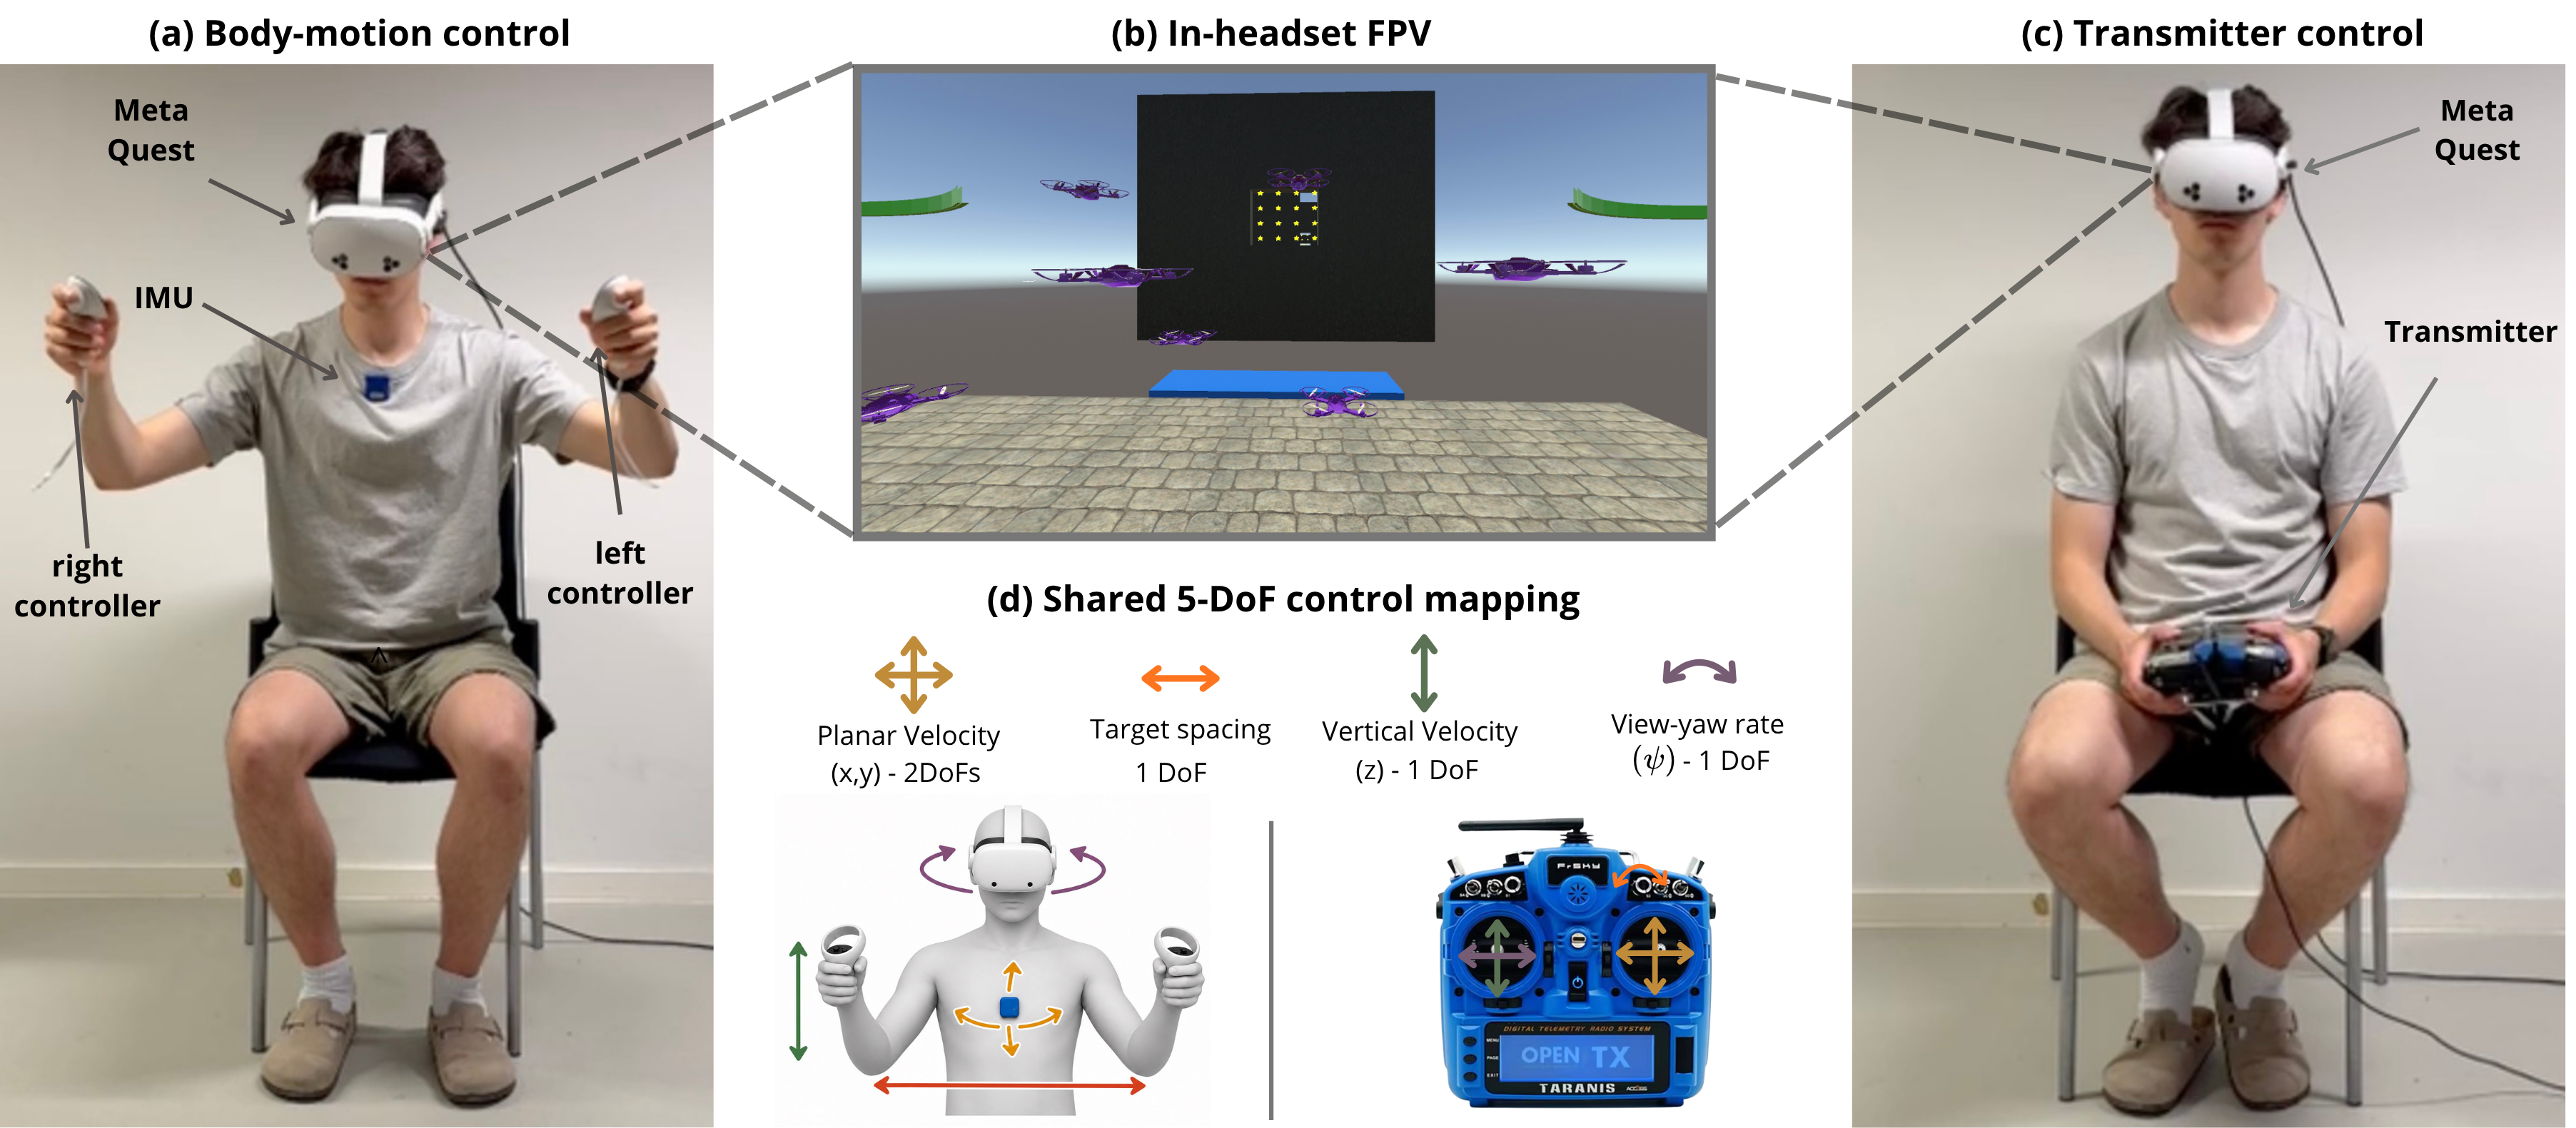
\includegraphics[width=\textwidth]{Figures/carre.png}
%DIFDELCMD < %%%
%DIFDELCMD < \caption{%
{%DIFAUXCMD
\DIFdelFL{Overview of the within-subject experiment: (a) body-motion control,
(b) the in-headset rear-focal FPV view, (c) transmitter control, and
(d) the common five-DOF command set exposed by both interfaces: planar
velocity, vertical velocity, target spacing, and view-yaw rate.}}
%DIFAUXCMD
%DIFDELCMD < \label{fig:study_overview}
%DIFDELCMD < \end{figure*}
%DIFDELCMD < 

%DIFDELCMD < %%%
\DIFdelend \begin{abstract}
\DIFdelbegin \DIFdel{Aerial-swarm teleoperation from an immersive first-person view (FPV) requires continuous }\DIFdelend \DIFaddbegin \DIFadd{Immersive first-person-view teleoperation of aerial swarms requires concurrent
}\DIFaddend control of collective motion, view direction, and formation size. We \DIFdelbegin \DIFdel{present }\DIFdelend \DIFaddbegin \DIFadd{developed
}\DIFaddend a participant-calibrated upper-body interface \DIFdelbegin \DIFdel{for five-degree-of-
freedom control of a simulated aerial swarm. Torso inclination, controller
height and separation}\DIFdelend \DIFaddbegin \DIFadd{that mapped torso, hand}\DIFaddend , and head
\DIFdelbegin \DIFdel{yaw command planar velocity, vertical velocity,
inter-agent spacing, and view-yaw rate}\DIFdelend \DIFaddbegin \DIFadd{movements to five swarm DOF}\DIFaddend . In a within-subject study, 14 participants
navigated a \DIFaddbegin \DIFadd{simulated }\DIFaddend 15-agent swarm through three-dimensional obstacle courses
using body motion and a conventional transmitter. \DIFdelbegin \DIFdel{The complete
body-motion system }\DIFdelend \DIFaddbegin \DIFadd{Compared with transmitter
control, body motion }\DIFaddend reduced completion time by 19.4\%\DIFdelbegin \DIFdel{and centroid travel
distance }\DIFdelend \DIFaddbegin \DIFadd{, centroid path length }\DIFaddend by
7.0\%\DIFdelbegin \DIFdel{. An exploratory trajectory analysis also found 8.6\% less
three-dimensional cross-track motion. Delivered-command variation was lower
with body motion, although this comparison included interface-specific
filtering}\DIFdelend \DIFaddbegin \DIFadd{, and delivered-command variation by 88.8\%, while increasing path
directness and multi-DOF coordination}\DIFaddend . No clear differences were detected in
\DIFdelbegin \DIFdel{task accuracy, swarm
integrity, }\DIFdelend \DIFaddbegin \DIFadd{gate-centering error, collection yield, crash or disconnection counts, }\DIFaddend overall
workload, or usability\DIFdelbegin \DIFdel{, whereas physical }\DIFdelend \DIFaddbegin \DIFadd{. Physical }\DIFaddend demand was higher with body motion for all
participants. \DIFdelbegin \DIFdel{These findings demonstrate a
task-specific efficiency advantage for the implemented body-motion system,
without isolating the effects of input modality, command mapping, or signal
processing}\DIFdelend \DIFaddbegin \DIFadd{The implemented mapping therefore improved FPV navigation
efficiency at the cost of greater physical demand}\DIFaddend .
\end{abstract}

% =====================================================================
\DIFdelbegin \section{\DIFdel{Introduction}}
%DIFAUXCMD
\addtocounter{section}{-1}%DIFAUXCMD
\DIFdelend 

\DIFaddbegin \section{\DIFadd{Introduction}}
\DIFaddend Aerial swarms can extend sensing and coverage\DIFdelbegin \DIFdel{by coordinating many robots}\DIFdelend , but missions \DIFdelbegin \DIFdel{that depend on }\DIFdelend \DIFaddbegin \DIFadd{requiring }\DIFaddend human
judgment still \DIFdelbegin \DIFdel{require an }\DIFdelend \DIFaddbegin \DIFadd{need an effective }\DIFaddend interface between one operator and the
collective\DIFdelbegin \DIFdel{\mbox{%DIFAUXCMD
\cite{kolling2016survey,ben_focaldrone}}\hskip0pt%DIFAUXCMD
}\DIFdelend \DIFaddbegin \DIFadd{~\mbox{%DIFAUXCMD
\cite{kolling2016survey,hocraffer2017meta}}\hskip0pt%DIFAUXCMD
}\DIFaddend . Rather than command
\DIFdelbegin \DIFdel{agents
individually}\DIFdelend \DIFaddbegin \DIFadd{individual agents}\DIFaddend , the operator can \DIFdelbegin \DIFdel{specify low-dimensional commands for collective
motion. The present task requires five continuous command dimensions: forward and
lateral velocity, vertical velocity, view yaw rate, and formation spacing.
}\DIFdelend \DIFaddbegin \DIFadd{steer the swarm through collective
commands. In three-dimensional environments, passing through an opening may
require concurrent changes in planar translation, altitude, formation spacing,
and view direction. The interface must therefore support these DOF together
rather than sequentially.
}\DIFaddend 

\DIFdelbegin \DIFdel{An external view, such as a }\DIFdelend \DIFaddbegin \DIFadd{Viewpoint further constrains control. A }\DIFaddend top-down view (TDV) \DIFdelbegin \DIFdel{, exposes swarmgeometry, whereas a focal-agent }\DIFdelend \DIFaddbegin \DIFadd{reveals the swarm's
spatial extent, connectivity, and relationship to nearby obstacles. However, it
requires an external viewing platform or real-time scene reconstruction. The
former can introduce a single point of failure, while the latter adds
computation and sensing requirements. A }\DIFaddend first-person view (FPV) can \DIFdelbegin \DIFdel{be obtained from an onboard camera
without a dedicated viewing
platform. This advantage comes with restricted global awareness, a viewpoint
that movesor transfers between agents, and a command frame that rotateswith
the view \mbox{%DIFAUXCMD
\cite{ben_focaldrone,macchini2021impact}}\hskip0pt%DIFAUXCMD
. FPV yaw must therefore be
controlled together with swarm translation}\DIFdelend \DIFaddbegin \DIFadd{instead be
streamed from a }\emph{\DIFadd{focal agent}}\DIFadd{, the swarm member whose onboard camera
currently supplies the operator's view. The source can transfer if that agent
becomes unavailable~\mbox{%DIFAUXCMD
\cite{ben_focaldrone}}\hskip0pt%DIFAUXCMD
. However, the limited field of view
and occlusions hide parts of the swarm and environment, while the viewpoint
moves}\DIFaddend , \DIFdelbegin \DIFdel{altitude, and spacing.
}\DIFdelend \DIFaddbegin \DIFadd{rotates, and may transfer between agents. FPV therefore limits global
awareness while the operator coordinates several swarm DOF.
}\DIFaddend 

\DIFdelbegin \textit{\DIFdel{Jarvis et al.}}%DIFAUXCMD
\DIFdel{'s interface assigned these commands to two
transmitter }\DIFdelend \DIFaddbegin \begin{figure}[!t]
\centering
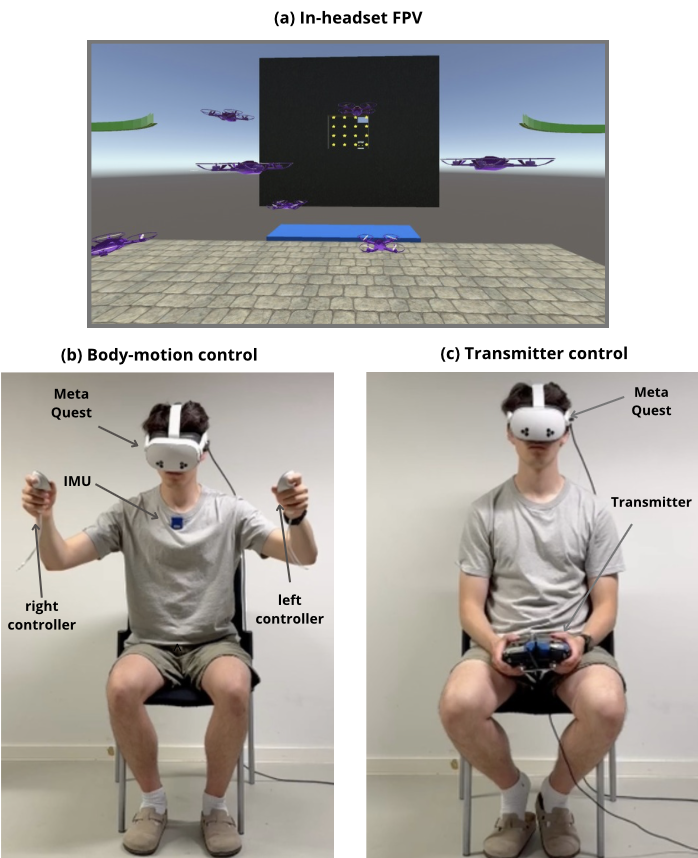
\includegraphics[width=\columnwidth]{Figures/111.png}
\caption{\DIFaddFL{Experimental interfaces and common visual feedback:
(a) the in-headset rear-focal FPV view, (b) body-motion control using
a torso-mounted IMU and hand controllers, and (c) transmitter control.
Both conditions used the same headset, visual feedback, and swarm
command space.}}
\label{fig:study_overview}
\end{figure}

\DIFadd{Jarvis et al.\ demonstrated rear-focal FPV swarm teleoperation and compared
different onboard viewpoints~\mbox{%DIFAUXCMD
\cite{ben_focaldrone}}\hskip0pt%DIFAUXCMD
. Their transmitter mapped
planar translation, vertical motion, view yaw, and formation spacing to two
}\DIFaddend sticks and a rotary \DIFdelbegin \DIFdel{control \mbox{%DIFAUXCMD
\cite{ben_focaldrone}}\hskip0pt%DIFAUXCMD
. Although
familiar, this layout may serialize adjustments when several dimensions must
change during the same maneuver. Studies of multidimensional input distinguish
such separable operation from integral input}\DIFdelend \DIFaddbegin \DIFadd{knob. However, it remains unclear whether this layout is
well suited to the concurrent adjustment of five continuous DOF.
Multidimensional-input research distinguishes separable control, in which
dimensions are adjusted independently, from integral control}\DIFaddend , in which \DIFdelbegin \DIFdel{dimensions can
be varied
concurrently \mbox{%DIFAUXCMD
\cite{jacob1994integrality,zhai1998quantifying}}\hskip0pt%DIFAUXCMD
. }\DIFdelend \DIFaddbegin \DIFadd{they can
vary together~\mbox{%DIFAUXCMD
\cite{jacob1994integrality,zhai1998quantifying}}\hskip0pt%DIFAUXCMD
. Splitting five
commands across two sticks and a knob may therefore impede simultaneous
adjustment.
}

\DIFaddend An upper-body interface \DIFdelbegin \DIFdel{could instead distribute }\DIFdelend \DIFaddbegin \DIFadd{can instead distribute spatially corresponding }\DIFaddend commands
across the head, torso, and \DIFdelbegin \DIFdel{arms
while preserving spatial correspondence between torso inclination and planar
motion in the focal agent's yaw frame. }%DIFDELCMD < 

%DIFDELCMD < %%%
\DIFdel{Prior body--machine interfaces have enabled immersive or }\DIFdelend \DIFaddbegin \DIFadd{hands. Body--machine interfaces have already enabled
immersive and }\DIFaddend personalized control of individual drones
\DIFdelbegin \DIFdel{\mbox{%DIFAUXCMD
\cite{rognon2018flyjacket,miehlbradt2018datadriven,macchini2024datadriven}}\hskip0pt%DIFAUXCMD
. }\DIFdelend \DIFaddbegin \DIFadd{\mbox{%DIFAUXCMD
\cite{rognon2018flyjacket,miehlbradt2018datadriven,
macchini2024datadriven}}\hskip0pt%DIFAUXCMD
. Macchini et al.\ found that robots with
more DOF elicited the use of more body segments and greater variation in motion
strategies across users, increasing the need for personalized mappings
\mbox{%DIFAUXCMD
\cite{macchini2024datadriven}}\hskip0pt%DIFAUXCMD
. This result motivates a participant-calibrated
interface for the present five-DOF task. }\DIFaddend At swarm level, personalized \DIFdelbegin \DIFdel{hand-motion mappings controlled four dimensions
}\DIFdelend \DIFaddbegin \DIFadd{hand
motion has supported four-dimensional control }\DIFaddend from an external view\DIFaddbegin \DIFadd{point}\DIFaddend  \cite{macchini2021personalized}, while tactile and gesture-based \DIFdelbegin \DIFdel{interfaces supported hand-guided swarm motion and aerial-formation
}\DIFdelend \DIFaddbegin \DIFadd{systems have
supported other forms of swarm and formation }\DIFaddend control
\cite{tsykunov2019swarmtouch,kratky2025gesture}. \DIFdelbegin \DIFdel{Conversely, }\DIFdelend \DIFaddbegin \DIFadd{Together, these studies support multidimensional body control but do not establish its effectiveness for a swarm viewed through a moving focal agent. 
}

\DIFadd{We therefore investigate whether distributing five continuous swarm commands
across the head, torso, and hands can address the input bottleneck of
}\DIFaddend focal-agent \DIFdelbegin \DIFdel{FPV swarm control has been studied using a conventional transmitter
\mbox{%DIFAUXCMD
\cite{ben_focaldrone}}\hskip0pt%DIFAUXCMD
. 
These studies leave open whether upper-body motion can
support continuous control of swarm translation, altitude, formation spacing,
and view yaw from within the group. }%DIFDELCMD < 

%DIFDELCMD < %%%
\DIFdel{We address this question with }\DIFdelend \DIFaddbegin \DIFadd{FPV swarm teleoperation. We implement }\DIFaddend a participant-calibrated \DIFdelbegin \DIFdel{upper-body interface for
a simulated swarm. Torso }\DIFdelend \DIFaddbegin \DIFadd{interface in which torso }\DIFaddend inclination commands planar velocity, mean hand height commands vertical velocity, hand separation \DIFdelbegin \DIFdel{sets target inter-agent }\DIFdelend \DIFaddbegin \DIFadd{commands formation }\DIFaddend spacing, and head yaw commands FPV yaw rate. We compare the \DIFdelbegin \DIFdel{complete }\DIFdelend interface with a \DIFdelbegin \DIFdel{radio-control }\DIFdelend \DIFaddbegin \DIFadd{conventional drone }\DIFaddend transmitter in a
within-subject study of 14 participants navigating \DIFaddbegin \DIFadd{a simulated swarm through
}\DIFaddend three-dimensional \DIFdelbegin \DIFdel{gap-passing }\DIFdelend \DIFaddbegin \DIFadd{obstacle }\DIFaddend courses. The \DIFdelbegin \DIFdel{study evaluates traversal efficiency, trajectory geometry,
delivered-command variation, task accuracy, swarm integrity, workload,
usability, and preference. Our }\DIFdelend contributions are (i) a \DIFdelbegin \DIFdel{five-dimensional body-motion }\DIFdelend \DIFaddbegin \DIFadd{five-DOF
upper-body }\DIFaddend mapping aligned with the \DIFdelbegin \DIFdel{focal agent's yaw frame , including during viewpoint }\DIFdelend \DIFaddbegin \DIFadd{focal-agent reference frame during view
}\DIFaddend rotation and transfer, and (ii) a \DIFdelbegin \DIFdel{user study showing faster and more direct traversal without
detected differences in task accuracy, swarm integrity, overall workload, or
usability, but with higher physical demand}\DIFdelend \DIFaddbegin \DIFadd{within-subject evaluation of navigation
efficiency, command behavior, task outcomes, and user experience}\DIFaddend .

%DIF <  =====================================================================
\section{Swarm Control System and Input Interfaces}
% --- 2a. Methodology: the interface and the body-to-swarm mapping ---

\subsection{Shared Swarm and FPV System}
\label{sec:system}
\DIFdelbegin %DIFDELCMD < 

%DIFDELCMD < %%%
\DIFdelend Both input conditions generated a common five-dimensional command vector for the simulated 15-agent swarm:
\begin{equation}
\mathbf{u}_t =
\left[
v_{\mathrm{fwd},t}^{\mathrm{ref}},
v_{\mathrm{lat},t}^{\mathrm{ref}},
v_{\mathrm{vert},t}^{\mathrm{ref}},
\dot{\psi}_{t}^{\mathrm{cmd}},
\rho_t^{*}
\right]^{\mathsf T}.
\label{eq:swarm_command}
\end{equation}
The first three components specify focal-frame horizontal and \DIFdelbegin \DIFdel{world-vertical
reference velocities, $\dot{\psi}_{t}^{\mathrm{cmd}}$ specifies }\DIFdelend \DIFaddbegin \DIFadd{world-frame vertical velocities; the remaining components specify }\DIFaddend FPV yaw rate \DIFdelbegin \DIFdel{,
and $\rho_t^{*}$ specifies absolute target surface-to-surface clearance}\DIFdelend \DIFaddbegin \DIFadd{and target agent spacing}\DIFaddend .

A decentralized Olfati--Saber controller~\cite{olfatisaber2006flocking}
combined \DIFdelbegin \DIFdel{clearance }\DIFdelend \DIFaddbegin \DIFadd{spacing }\DIFaddend regulation, velocity alignment, reference-velocity tracking,
and obstacle repulsion. \DIFdelbegin \DIFdel{At 50~Hz, }\DIFdelend \DIFaddbegin \DIFadd{Surviving agents formed }\DIFaddend an undirected interaction
graph\DIFdelbegin \DIFdel{connected agents separated by less than
$R_t=\max(2\rho_t^{*},\,\rho_t^{*}+2~\mathrm{m})$; the component containing
the focal agent defined the controlled swarm. Following Jarvis }\DIFdelend \DIFaddbegin \DIFadd{, with an edge between agents whose Euclidean separation was below
}\[
\DIFadd{R_t=\max(2\rho_t^*,\,\rho_t^*+2~\mathrm{m}).
}\]
\DIFadd{The largest connected component defined the connected swarm; surviving agents
outside it were classified as disconnected. The simulation built on the FPV
swarm-teleoperation framework of Palle }\DIFaddend et al.~\DIFdelbegin \DIFdel{\mbox{%DIFAUXCMD
\cite{ben_focaldrone}}\hskip0pt%DIFAUXCMD
, the agent farthest rearward along the current
}\DIFdelend \DIFaddbegin \DIFadd{\mbox{%DIFAUXCMD
\cite{palle2026multisensory}}\hskip0pt%DIFAUXCMD
.
}

\DIFadd{To isolate input-interface effects, both conditions used the rear-focal
stereoscopic FPV of Jarvis et al., which keeps most agents ahead of the camera
and outperformed front and multiple-view configurations~\mbox{%DIFAUXCMD
\cite{ben_focaldrone}}\hskip0pt%DIFAUXCMD
.
The agent furthest back along the }\DIFaddend horizontal viewing direction provided the
\DIFdelbegin \DIFdel{stereoscopic FPV. A }\DIFdelend \DIFaddbegin \DIFadd{feed; }\DIFaddend handoff occurred only when another \DIFdelbegin \DIFdel{candidate }\DIFdelend \DIFaddbegin \DIFadd{agent }\DIFaddend remained at least 0.5~m \DIFdelbegin \DIFdel{farther rearward }\DIFdelend \DIFaddbegin \DIFadd{further
back }\DIFaddend for 0.5~s\DIFaddbegin \DIFadd{.
}\DIFaddend 

In both conditions, participants viewed the FPV through a virtual reality (VR)
headset (Meta Quest 3S\DIFaddbegin \DIFadd{, Meta, USA}\DIFaddend ). For body-motion control, the headset measured
head yaw, \DIFdelbegin \DIFdel{the }\DIFdelend two handheld controllers \DIFdelbegin \DIFdel{connected to the headset measured three-dimensional }\DIFdelend \DIFaddbegin \DIFadd{measured }\DIFaddend hand positions, and a chest-mounted
inertial measurement unit (LPMS-B2\DIFdelbegin \DIFdel{IMU}\DIFdelend \DIFaddbegin \DIFadd{, LP-Research, Japan}\DIFaddend ) measured torso
inclination. \DIFdelbegin \DIFdel{Input hardware, mapping, participant calibration, and signal processing were condition-specific; the }\DIFdelend \DIFaddbegin \DIFadd{The }\DIFaddend swarm controller, command limits, focal-agent logic, and
simulation were \DIFdelbegin \DIFdel{shared}\DIFdelend \DIFaddbegin \DIFadd{the same in both conditions; only the input hardware and
filtering differed}\DIFaddend .

\subsection{Body-to-Swarm Mapping}
\label{sec:mapping} 
\DIFaddbegin \DIFadd{The mapping followed four principles: (i) spatial correspondence between body
and swarm motion, (ii) distribution of commands across body segments to reduce
input competition and permit concurrent control, (iii) control semantics
matched to each command, and (iv) participant-specific calibration.
}\DIFaddend 

At time $t$, the interface measured sagittal and lateral torso inclination
$(\theta_t,\phi_t)$, headset yaw $\psi_t$, mean controller height
\[
h_t=\frac{y^W_{L,t}+y^W_{R,t}}{2},
\]
and controller separation
\[
s_t=\left\lVert\mathbf{p}^W_{R,t}-\mathbf{p}^W_{L,t}\right\rVert .
\]
\DIFaddbegin 

\DIFaddend Translation and yaw \DIFdelbegin \DIFdel{were rate controlled}\DIFdelend \DIFaddbegin \DIFadd{used rate control}\DIFaddend , so a sustained posture produced
continuous motion\DIFdelbegin \DIFdel{, whereas controller separation mapped directly to the desired formation clearance}\DIFdelend \DIFaddbegin \DIFadd{; hand separation directly set target agent spacing}\DIFaddend .

\emph{Participant-specific normalization:}
Each rate-controlled signal was mapped to $[-1,1]$ using its calibrated lower
extreme, neutral value, and upper extreme $(q^{-},q^{0},q^{+})$, with a
deadzone of half-width $d$ around neutral. Let
$q_{\mathrm{L}}=q^{0}-d$ and $q_{\mathrm{U}}=q^{0}+d$. The normalization was
\begin{equation}
\mathcal{D}(q_t;q^{-},q^{0},q^{+},d)=
\begin{cases}
\displaystyle
\max\!\left(-1,
\frac{q_t-q_{\mathrm{L}}}{q_{\mathrm{L}}-q^{-}}\right),
& q_t<q_{\mathrm{L}},\\[6pt]
0,
& q_{\mathrm{L}}\leq q_t\leq q_{\mathrm{U}},\\[3pt]
\displaystyle
\min\!\left(1,
\frac{q_t-q_{\mathrm{U}}}{q^{+}-q_{\mathrm{U}}}\right),
& q_t>q_{\mathrm{U}}.
\end{cases}
\label{eq:deadzone_mapping}
\end{equation}
Separate scaling on either side of neutral accommodated asymmetric ranges of
motion.

\DIFdelbegin %DIFDELCMD < \begin{figure}[!t]
%DIFDELCMD < %%%
\DIFdelendFL \DIFaddbeginFL \begin{figure*}[!t]
\DIFaddendFL \centering
\DIFdelbeginFL %DIFDELCMD < 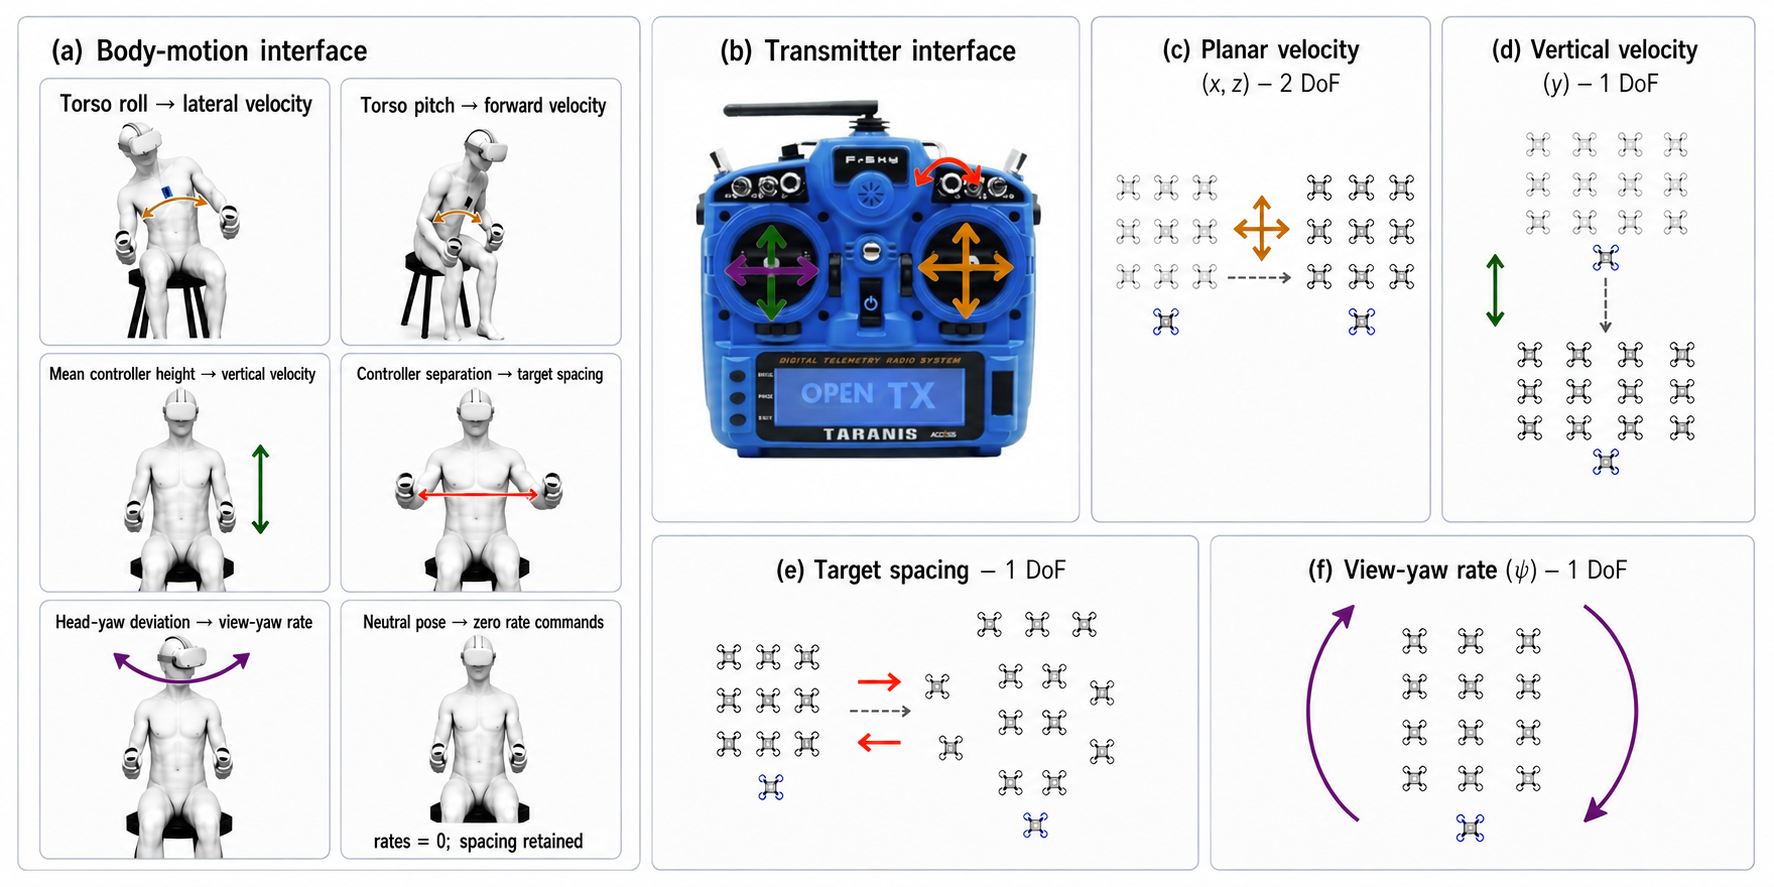
\includegraphics[width=\linewidth]{Figures/hom.png}
%DIFDELCMD < %%%
\DIFdelendFL \DIFaddbeginFL 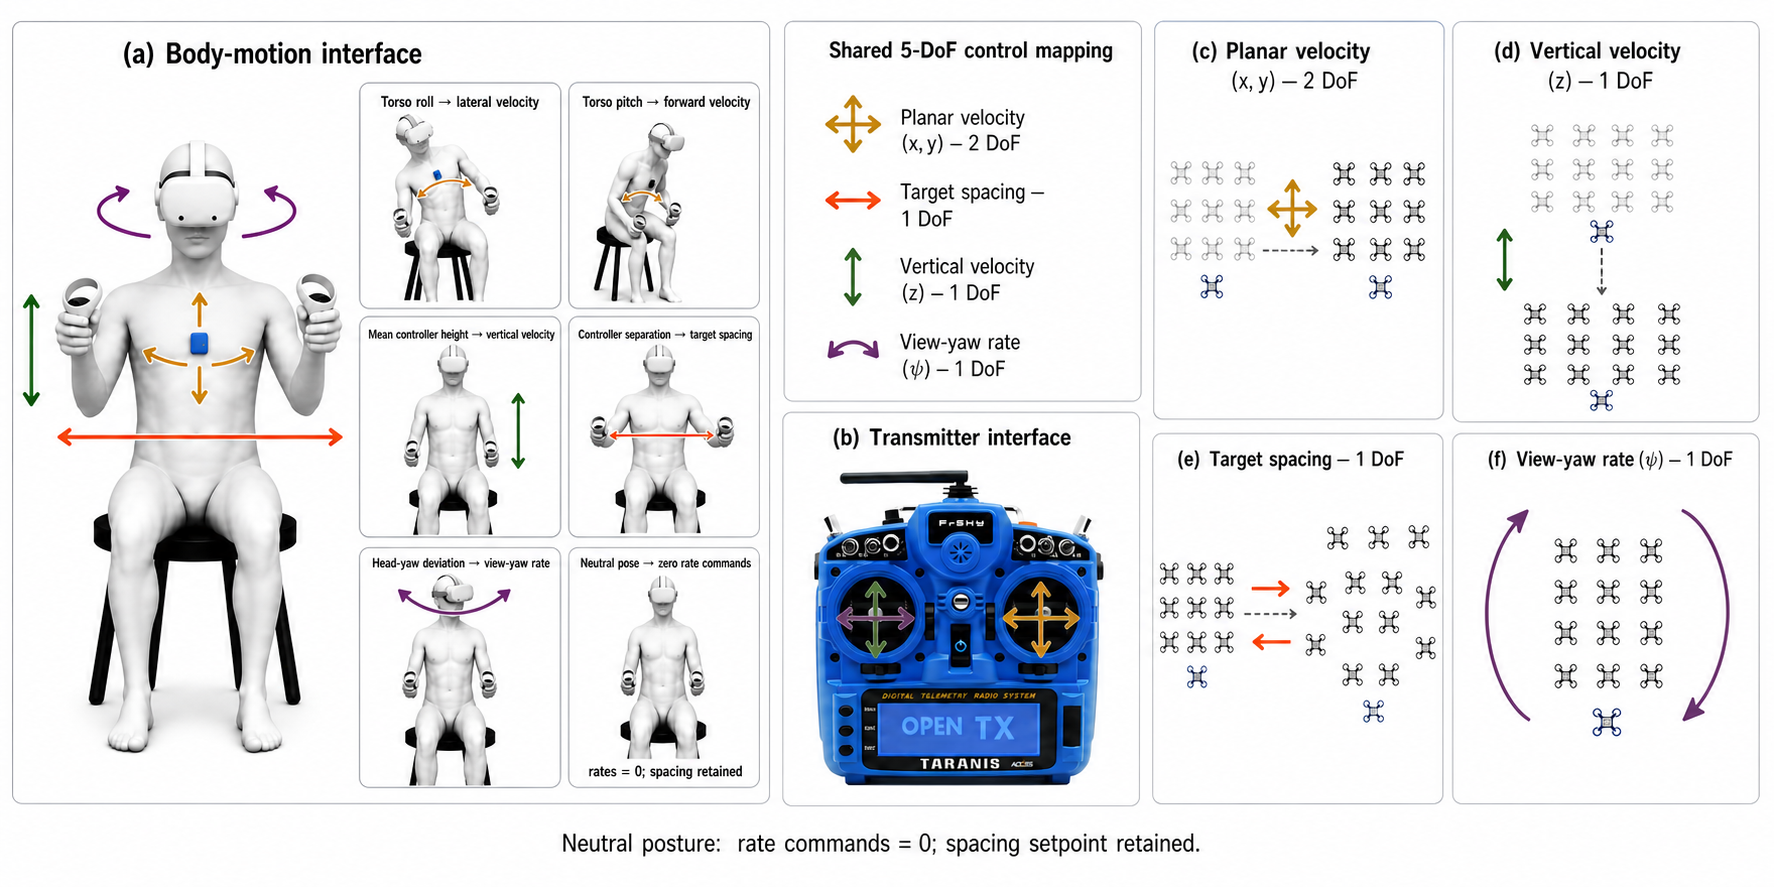
\includegraphics[width=\textwidth]{Figures/l.png}
\DIFaddendFL \caption{Body-to-swarm \DIFdelbeginFL \DIFdelFL{control }\DIFdelendFL mappings\DIFdelbeginFL \DIFdelFL{: }\DIFdelendFL \DIFaddbeginFL \DIFaddFL{. Panels }\DIFaddendFL (a)\DIFdelbeginFL \DIFdelFL{torso roll controls lateral
velocity, }\DIFdelendFL \DIFaddbeginFL \DIFaddFL{--}\DIFaddendFL (\DIFdelbeginFL \DIFdelFL{b) torso pitch controls forward velocity, (c) mean controller
height controls vertical velocity, (d) controller separation controls target
spacing, and (}\DIFdelendFL e) \DIFdelbeginFL \DIFdelFL{head-yaw deviation controls view-yaw rate. }\DIFdelendFL \DIFaddbeginFL \DIFaddFL{show the posture or hand
movement assigned to each command; }\DIFaddendFL (f) \DIFdelbeginFL \DIFdelFL{The }\DIFdelendFL \DIFaddbeginFL \DIFaddFL{shows the }\DIFaddendFL neutral pose\DIFdelbeginFL \DIFdelFL{produces zero rate commands }\DIFdelendFL \DIFaddbeginFL \DIFaddFL{, which stops
motion }\DIFaddendFL while retaining the \DIFdelbeginFL \DIFdelFL{current target-spacing
}\DIFdelendFL \DIFaddbeginFL \DIFaddFL{spacing }\DIFaddendFL setpoint. Faded formations \DIFdelbeginFL \DIFdelFL{illustrate }\DIFdelendFL \DIFaddbeginFL \DIFaddFL{indicate }\DIFaddendFL the
\DIFdelbeginFL \DIFdelFL{direction of the }\DIFdelendFL commanded \DIFdelbeginFL \DIFdelFL{swarm
motion}\DIFdelendFL \DIFaddbeginFL \DIFaddFL{direction}\DIFaddendFL , scaling, or view rotation.}
\label{fig:mapping}
\DIFdelbeginFL %DIFDELCMD < \end{figure}
%DIFDELCMD < %%%
\DIFdelend \DIFaddbegin \end{figure*}
\DIFaddend 




\emph{Translation:}
The normalized translation commands were
\begin{align}
c_{\mathrm{fwd},t}
&=\mathcal{D}(\theta_t;\theta^{-},0,\theta^{+},5^{\circ}),
\nonumber\\
c_{\mathrm{lat},t}
&=\mathcal{D}(\phi_t;\phi^{-},0,\phi^{+},5^{\circ}),
\nonumber\\
c_{\mathrm{vert},t}
&=\mathcal{D}(h_t;h_{\min},h_0,h_{\max},0.05~\mathrm{m}).
\label{eq:body_rate_commands}
\end{align}
Positive \DIFdelbegin \DIFdel{commands denoted }\DIFdelend \DIFaddbegin \DIFadd{values commanded }\DIFaddend forward, rightward, and upward motion. \DIFdelbegin \DIFdel{The }\DIFdelend \DIFaddbegin \DIFadd{After
smoothing, the }\DIFaddend normalized commands were \DIFdelbegin \DIFdel{smoothed, with the resulting values denoted by
$(\bar c_{\mathrm{fwd},t},\bar c_{\mathrm{lat},t},
\bar c_{\mathrm{vert},t})$. These values were then scaled by
}\DIFdelend \DIFaddbegin \DIFadd{multiplied by
}\DIFaddend $10~\mathrm{m\,s^{-1}}$ to obtain the \DIFdelbegin \DIFdel{corresponding reference velocities $(v_{\mathrm{fwd},t}^{\mathrm{ref}},v_{\mathrm{lat},t}^{\mathrm{ref}},
v_{\mathrm{vert},t}^{\mathrm{ref}})$ }\DIFdelend \DIFaddbegin \DIFadd{reference velocities }\DIFaddend in
Eq.~\eqref{eq:swarm_command}.
\DIFdelbegin \DIFdel{The forward and lateral velocities were defined relative to the displayed
heading and updated after FPV rotation or viewpoint transfer.
}\DIFdelend 

%DIF >  The forward and lateral velocities were defined relative to the displayed
%DIF >  heading and updated after FPV rotation or viewpoint transfer.
\DIFaddbegin 

\DIFaddend \emph{Inter-agent spacing:}
Controller separation \DIFdelbegin \DIFdel{$s_t$ was linearly mapped from the participant-specific
range }\DIFdelend \DIFaddbegin \DIFadd{was mapped linearly from }\DIFaddend $[s_{\min},s_{\max}]$ to \DIFdelbegin \DIFdel{a target
surface-to-surface clearance
}\DIFdelend \DIFaddbegin \DIFadd{target
agent spacing }\DIFaddend $\rho_t\in[1,5]~\mathrm{m}$\DIFdelbegin \DIFdel{. The mapping was clipped at the calibrated limits }\DIFdelend \DIFaddbegin \DIFadd{, then clipped }\DIFaddend and smoothed to produce
the applied command $\rho_t^*$\DIFdelbegin \DIFdel{in
Eq.
~\eqref{eq:swarm_command}. Because this was an absolute mapping,
participants selected the desired clearance directly rather than commanding
an expansion or contraction rate.
}\DIFdelend \DIFaddbegin \DIFadd{.
}\DIFaddend 

\emph{FPV yaw:}
With
$\Delta\psi_t=
\operatorname{wrap}_{[-180^{\circ},180^{\circ})}
(\psi_t-\psi_{0,t})$
denoting the head-yaw deviation from its neutral orientation, the FPV yaw-rate
command was
\begin{equation}
\dot{\psi}^{\,\mathrm{cmd}}_t
=
48^{\circ}\mathrm{s}^{-1}
\mathcal{D}\!\left(
\Delta\psi_t;\psi_{\mathrm{L}},0,\psi_{\mathrm{R}},10^{\circ}
\right).
\label{eq:yaw_rate}
\end{equation}
Returning the head to neutral stopped FPV rotation without restoring the
previous viewing direction.
\DIFdelbegin \DIFdel{The neutral yaw was slowly adapted during periods
of head stillness to compensate for postural drift. No additional yaw
smoothing was applied.
}\DIFdelend 

\DIFdelbegin \DIFdel{The fixed gains, deadzones, and smoothing settings were selected through pilot
and informal testing}\DIFdelend \DIFaddbegin \DIFadd{Pilot testing was used to tune controller parameters and refine the
body-to-swarm mapping}\DIFaddend .

\subsection{Participant-Specific Calibration}
\label{sec:calibration}
\DIFdelbegin %DIFDELCMD < 

%DIFDELCMD < %%%
\DIFdelend Each participant completed a one-time guided 13-pose calibration to record
seated neutral postures and comfortable motion limits. The chair configuration and Quest tracking origin remained fixed thereafter.

Calibration included five torso poses (neutral and maximum forward, backward,
left, and right), three head-yaw poses (neutral and maximum left and right),
two controller-separation poses (minimum and maximum), and three
controller-height poses (minimum, neutral, and maximum). Neutral torso and head poses defined the IMU orientation offset and headset yaw
reference $\psi_0$, respectively; \DIFdelbegin \DIFdel{only $(s_{\min},s_{\max})$ parameterized the absolute spacing
mapping.
}\DIFdelend \DIFaddbegin \DIFadd{the controller-separation limits defined the
agent-spacing range.
}\DIFaddend 

\DIFdelbegin \DIFdel{The measured bounds directly parameterized the
translation, yaw-rate, and
spacing mappings.
}\DIFdelend Table~\ref{tab:calibration_summary} summarizes the \DIFdelbegin \DIFdel{resulting spans; angular
}\DIFdelend \DIFaddbegin \DIFadd{calibrated spans. Angular
}\DIFaddend spans combine opposing excursions, \DIFdelbegin \DIFdel{whereas }\DIFdelend \DIFaddbegin \DIFadd{while }\DIFaddend position spans are
maximum--minimum differences.

\DIFdelbegin %DIFDELCMD < \begin{table}[!tb]
%DIFDELCMD < %%%
\DIFdelendFL \DIFaddbeginFL \begin{table}[b]
\DIFaddendFL \centering
\caption{Calibrated input spans across participants ($N=14$).}
\label{tab:calibration_summary}
\footnotesize
\setlength{\tabcolsep}{3.5pt}
\begin{tabular}{@{}lcc@{}}
\toprule
Input span & Mean $\pm$ SD & Range \\
\midrule
Sagittal torso ($^\circ$)       & $56.4 \pm 18.4$  & $34.2$--$98.1$ \\
Lateral torso ($^\circ$)        & $52.0 \pm 18.0$  & $26.2$--$81.2$ \\
Head yaw ($^\circ$)             & $117.5 \pm 24.7$ & $65.6$--$138.0$ \\
Controller separation (m)       & $1.10 \pm 0.33$  & $0.70$--$1.51$ \\
Controller height (m)           & $0.77 \pm 0.22$  & $0.43$--$1.22$ \\
\bottomrule
\end{tabular}
\end{table}

\subsection{Transmitter Baseline}
\label{sec:transmitter}

A conventional \DIFdelbegin \DIFdel{radio-control transmitter (FrSky }\DIFdelend \DIFaddbegin \DIFadd{drone transmitter (}\DIFaddend Taranis X9D Plus\DIFdelbegin \DIFdel{) }\DIFdelend \DIFaddbegin \DIFadd{, FrSky, China) connected to
the PC by USB }\DIFaddend generated the same command vector \DIFdelbegin \DIFdel{, }\DIFdelend $\mathbf{u}_t$\DIFdelbegin \DIFdel{, as the body-motion interface}\DIFdelend . The right stick
controlled planar velocity, the left horizontal axis controlled FPV yaw rate,
the non-self-centering \DIFdelbegin \DIFdel{left }\DIFdelend throttle controlled vertical velocity, and the right
rotary knob set target \DIFdelbegin \DIFdel{inter-agent clearance}\DIFdelend \DIFaddbegin \DIFadd{agent spacing}\DIFaddend . Stick axes used \DIFdelbegin \DIFdel{a symmetric 0.12
deadzone with rescaling of the remaining range, while }\DIFdelend \DIFaddbegin \DIFadd{symmetric deadzones, and
}\DIFaddend the knob mapped linearly to $\rho^*\in[1,5]$~m. \DIFdelbegin \DIFdel{Both conditions used the same command limits and yaw-aligned reference frame. The transmitter received no participant-specific
calibration or additional temporal
filtering}\DIFdelend \DIFaddbegin \DIFadd{Pilot-tested gains and deadzones
were fixed across participants; no individual calibration or temporal
smoothing was applied}\DIFaddend .

% =====================================================================
\DIFdelbegin %DIFDELCMD < 

%DIFDELCMD < \label{sec:experiment}
%DIFDELCMD < 

%DIFDELCMD < %%%
\DIFdelend \section{Experimental Evaluation}
\label{sec:experiment}

\subsection{Participants and Study Design}
\label{sec:participants_design}

The study included $N=14$ adults recruited from the local university
community (10 men and 4 women; age: $22.4 \pm 4.0$ years, range 19--35).
\DIFdelbegin \DIFdel{Sample size reflected participant availability; no a priori power analysis was
conducted. Eligibility required }\DIFdelend \DIFaddbegin \DIFadd{Participants }\DIFaddend self-reported \DIFdelbegin \DIFdel{ability }\DIFdelend \DIFaddbegin \DIFadd{being able }\DIFaddend to perform the seated upper-body
movements and \DIFdelbegin \DIFdel{vision compatible with }\DIFdelend \DIFaddbegin \DIFadd{use }\DIFaddend the VR headset. All
participants completed the study, provided written informed consent, and were
compensated.

\DIFdelbegin \DIFdel{A }\DIFdelend \DIFaddbegin \DIFadd{We used a }\DIFaddend two-condition within-subject design\DIFdelbegin \DIFdel{compared the body-motion and transmitter
interfaces described in Sections~\ref{sec:system}--\ref{sec:transmitter}}\DIFdelend . The first participant's starting
interface was \DIFdelbegin \DIFdel{selected at random }\DIFdelend \DIFaddbegin \DIFadd{randomized }\DIFaddend and alternated thereafter, yielding seven participants
per sequence. \DIFdelbegin \DIFdel{Both conditions were
completed while seated during a single session lasting }\DIFdelend \DIFaddbegin \DIFadd{Sessions lasted }\DIFaddend approximately 1~h \DIFaddbegin \DIFadd{and were completed while
seated}\DIFaddend .

\subsection{Task and Procedure}
\label{sec:task}
\DIFdelbegin %DIFDELCMD < 

%DIFDELCMD < \begin{figure}[t]
%DIFDELCMD < \centering
%DIFDELCMD < 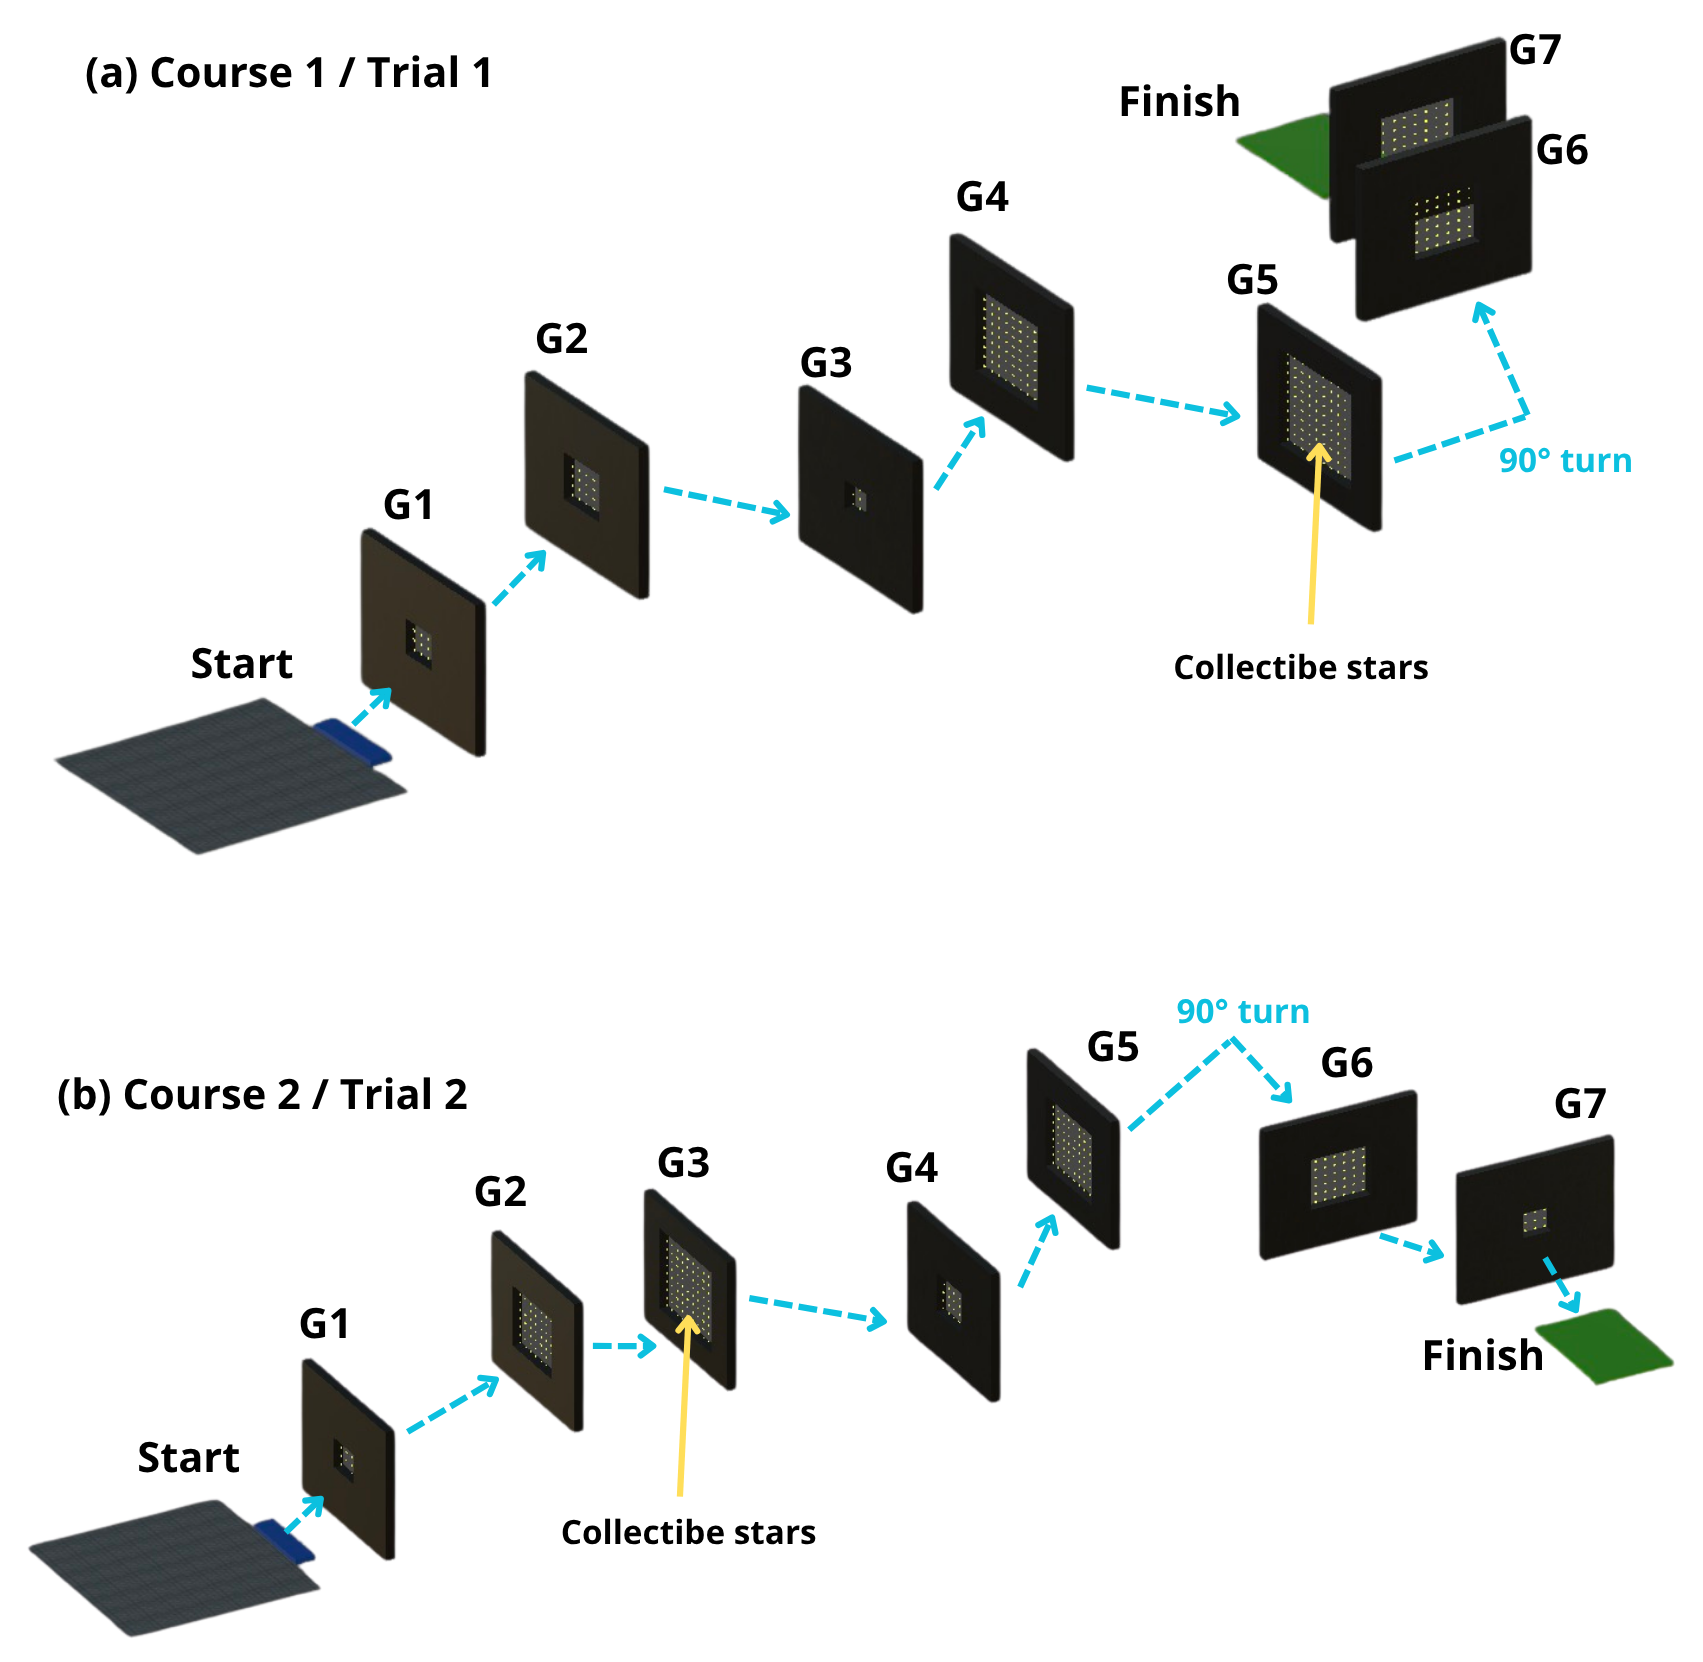
\includegraphics[width=\columnwidth]{Figures/layouts.png}
%DIFDELCMD < %%%
%DIFDELCMD < \caption{%
{%DIFAUXCMD
\DIFdelFL{Recorded-course layouts for (a) trial~1 and (b) trial~2.
Labels G1--G7 mark the gate sequence; dashed arrows show traversal direction.}}
%DIFAUXCMD
%DIFDELCMD < \label{fig:course_layouts}
%DIFDELCMD < \end{figure}
%DIFDELCMD < 

%DIFDELCMD < %%%
\DIFdel{All participants received identical }\DIFdelend \DIFaddbegin \DIFadd{All participants viewed the same }\DIFaddend prerecorded instructions and demonstrations.
They were \DIFdelbegin \DIFdel{asked }\DIFdelend \DIFaddbegin \DIFadd{instructed }\DIFaddend to complete each course \DIFdelbegin \DIFdel{as quicklyas possible while passing near the opening centers,
collecting }\DIFdelend \DIFaddbegin \DIFadd{quickly, pass near gate centers,
collect }\DIFaddend stars, and \DIFdelbegin \DIFdel{minimizing }\DIFdelend \DIFaddbegin \DIFadd{minimize }\DIFaddend crashes and disconnections. \DIFdelbegin \DIFdel{Control remained active during the approach, providing a flying start. Timing ran from the first agent crossing the start plane to the first agent crossing the finish plane. A run was valid only if the controlled-component centroid crossed all seven gate planes in sequence; no time limit was imposed. Participants viewed only }\DIFdelend \DIFaddbegin \DIFadd{They viewed only the
}\DIFaddend stereoscopic FPV, with no timer, score, or task-status display.

\DIFaddbegin \DIFadd{Each recorded course contained seven gates whose positions, heights, and
opening sizes were varied to require horizontal translation, altitude
adjustment, and formation-spacing control. Each course included one 90-degree turn, left in one course and right in the other, requiring participants to rotate the FPV and continue in the rotated focal-agent reference frame. Stars distributed across the gate openings encouraged control of swarm extent rather than only the focal agent or centroid; collection yield measured this collective performance.
}

\DIFaddend A star was collected when any agent entered its trigger\DIFdelbegin \DIFdel{; wall }\DIFdelend \DIFaddbegin \DIFadd{. Wall }\DIFaddend or inter-agent
collisions removed the affected agent, and \DIFdelbegin \DIFdel{survivors outside the interaction graph's }\DIFdelend \DIFaddbegin \DIFadd{surviving agents outside the }\DIFaddend largest
connected component were classified as disconnected at each sample.

Before the body-motion block, participants completed the calibration described
in Section~\ref{sec:calibration}. Each interface block began with familiarization
on the practice course: participants first maneuvered freely with standardized
experimenter guidance and then completed one unrecorded full-course traversal.
Two recorded runs followed in fixed order.

After each \DIFdelbegin \DIFdel{interface }\DIFdelend block, participants completed the weighted \DIFdelbegin \DIFdel{NASA Task Load
Index (}\DIFdelend NASA-TLX \DIFdelbegin \DIFdel{)~\mbox{%DIFAUXCMD
\cite{hart1988nasatlx} }\hskip0pt%DIFAUXCMD
and }\DIFdelend \DIFaddbegin \DIFadd{\mbox{%DIFAUXCMD
\cite{hart1988nasatlx} }\hskip0pt%DIFAUXCMD
and SUS~\mbox{%DIFAUXCMD
\cite{brooke1996sus} }\hskip0pt%DIFAUXCMD
for }\DIFaddend the \DIFdelbegin \DIFdel{10-item System Usability Scale
(SUS)~\mbox{%DIFAUXCMD
\cite{brooke1996sus} }\hskip0pt%DIFAUXCMD
, referring only to the }\DIFdelend two recorded runs.
After both blocks, they reported interface preference\DIFdelbegin \DIFdel{and }\DIFdelend \DIFaddbegin \DIFadd{, }\DIFaddend relative motion sickness\DIFdelbegin \DIFdel{(body motion,
transmitter, or no difference) and could provide optional free-text }\DIFdelend \DIFaddbegin \DIFadd{,
and optional }\DIFaddend comments.

\DIFdelbegin \subsection{\DIFdel{Outcome Measures}}
%DIFAUXCMD
\addtocounter{subsection}{-1}%DIFAUXCMD
\DIFdelend \DIFaddbegin \begin{figure}[t]
\centering
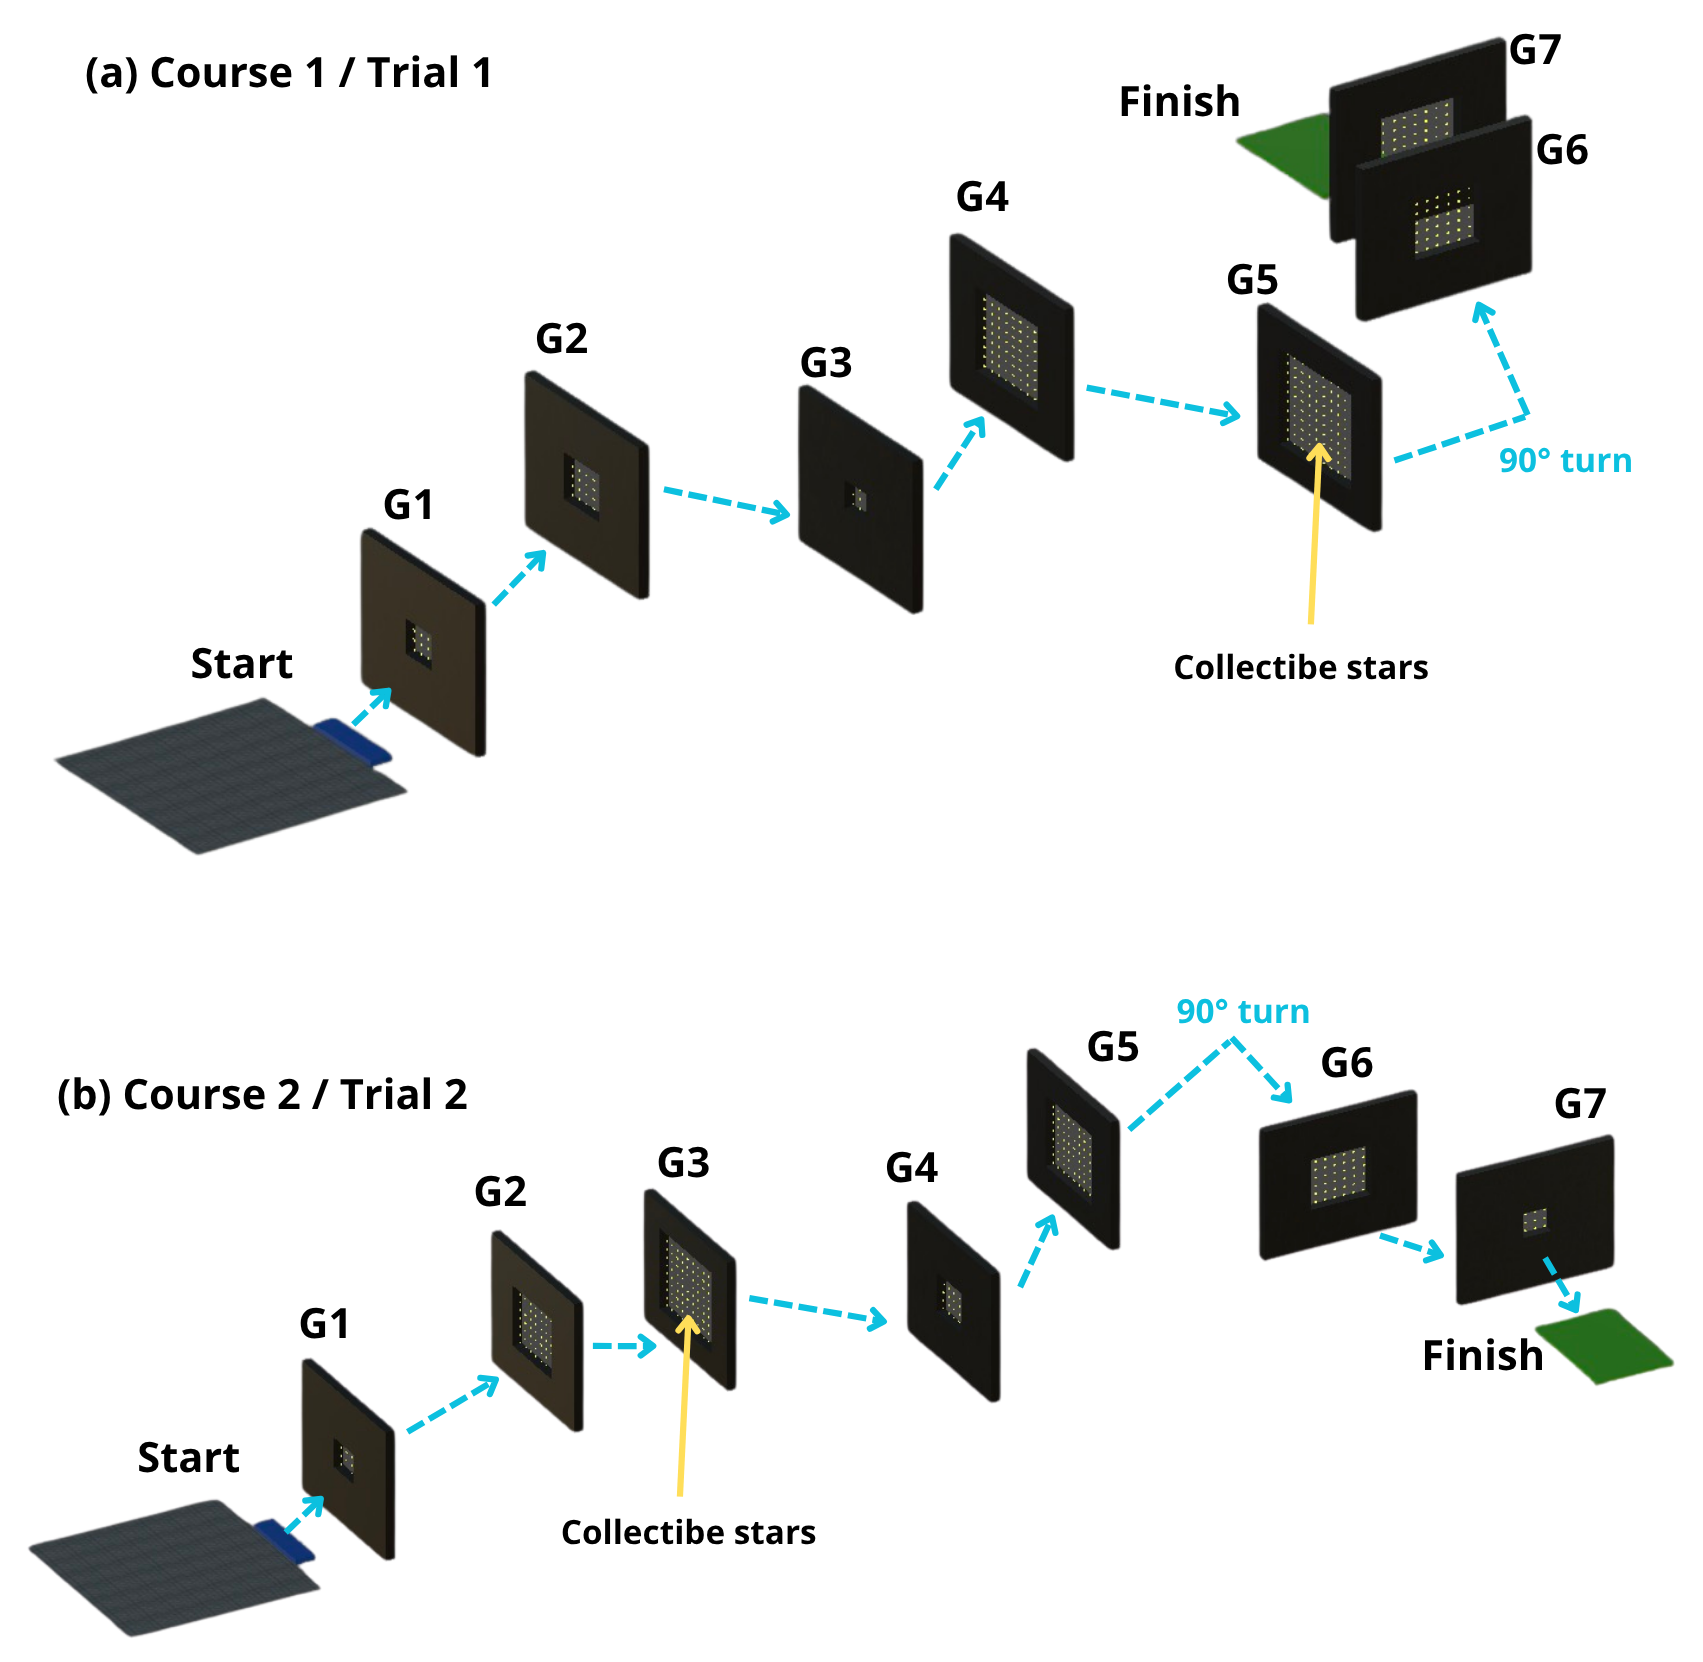
\includegraphics[width=\columnwidth]{Figures/layouts.png}
\caption{\DIFaddFL{Obstacle course layouts.
Labels G1--G7 mark the gate sequence; dashed arrows show traversal direction.}}
\label{fig:course_layouts}
\end{figure}
\DIFaddend 


\DIFdelbegin \DIFdel{We evaluated the interfaces in terms of }\textbf{\DIFdel{traversal efficiency}}%DIFAUXCMD
\DIFdel{, }\textbf{\DIFdel{movement
characteristics}}%DIFAUXCMD
\DIFdel{, }\textbf{\DIFdel{delivered-command behavior}}%DIFAUXCMD
\DIFdel{, }\textbf{\DIFdel{task performance and swarm
integrity}}%DIFAUXCMD
\DIFdel{, and }\textbf{\DIFdel{subjective experience}}%DIFAUXCMD
\DIFdelend \DIFaddbegin \subsection{\DIFadd{Evaluation Metrics}}
\DIFadd{Completion time was the primary outcome, consistent with task-oriented HRI
evaluation~\mbox{%DIFAUXCMD
\cite{steinfeld2006metrics}}\hskip0pt%DIFAUXCMD
. Secondary measures covered trajectory characteristics, task performance, swarm integrity, delivered commands, and subjective experience}\DIFaddend .

\emph{Traversal efficiency.}
Completion time $T$ \DIFdelbegin \DIFdel{was measured between }\DIFdelend \DIFaddbegin \DIFadd{extended from }\DIFaddend the recorded start \DIFdelbegin \DIFdel{and finish events
and served as the primary performance outcome}\DIFdelend \DIFaddbegin \DIFadd{event to the finish event}\DIFaddend .
Centroid path length $L$ was the \DIFdelbegin \DIFdel{cumulative }\DIFdelend \DIFaddbegin \DIFadd{total }\DIFaddend three-dimensional distance travelled by
the \DIFdelbegin \DIFdel{controlled component}\DIFdelend \DIFaddbegin \DIFadd{controlled-component centroid}\DIFaddend , and mean speed was \DIFdelbegin \DIFdel{computed as }\DIFdelend $\bar v=L/T$. \DIFdelbegin \DIFdel{Lower completion time and path
length
, and higher mean speed , indicated more efficient traversal}\DIFdelend \DIFaddbegin \DIFadd{Path length
and speed were treated as supporting outcomes}\DIFaddend .

\emph{\DIFdelbegin \DIFdel{Movement }\DIFdelend \DIFaddbegin \DIFadd{Trajectory }\DIFaddend characteristics.}
\DIFdelbegin \DIFdel{Movement continuity was characterized by the time spent below $0.5~\mathrm{m\,s^{-1}}$
and the number of low-speed episodes lasting at least $0.5$~s. Segment
straightness was defined as the summed endpoint-to-endpoint distance of the
}\DIFdelend \DIFaddbegin \DIFadd{Path directness was the sum of the straight-line endpoint distances across
}\DIFaddend eight course segments\DIFaddbegin \DIFadd{, }\DIFaddend divided by the \DIFdelbegin \DIFdel{corresponding centroid path length .
We further measured the fraction of incremental motion orthogonal to the direct
three-dimensional segment directions, $C_{\perp}$, and excess vertical travel,
}\DIFdelend \DIFaddbegin \DIFadd{total path length $L$
\mbox{%DIFAUXCMD
\cite{mavrogiannis2022socialmomentum}}\hskip0pt%DIFAUXCMD
:
}\begin{equation}
\DIFadd{D_{\mathrm{path}}
=
\frac{1}{L}
\sum_{j=1}^{8}
\left\|
\mathbf{x}_{j,\mathrm{end}}
-
\mathbf{x}_{j,\mathrm{start}}
\right\|_2.
\label{eq:path_directness}
}\end{equation}
\DIFadd{The eight segments ran from the start to the first gate, between consecutive
gates, and from the final gate to the finish.
}


\begin{figure*}[t]
\centering
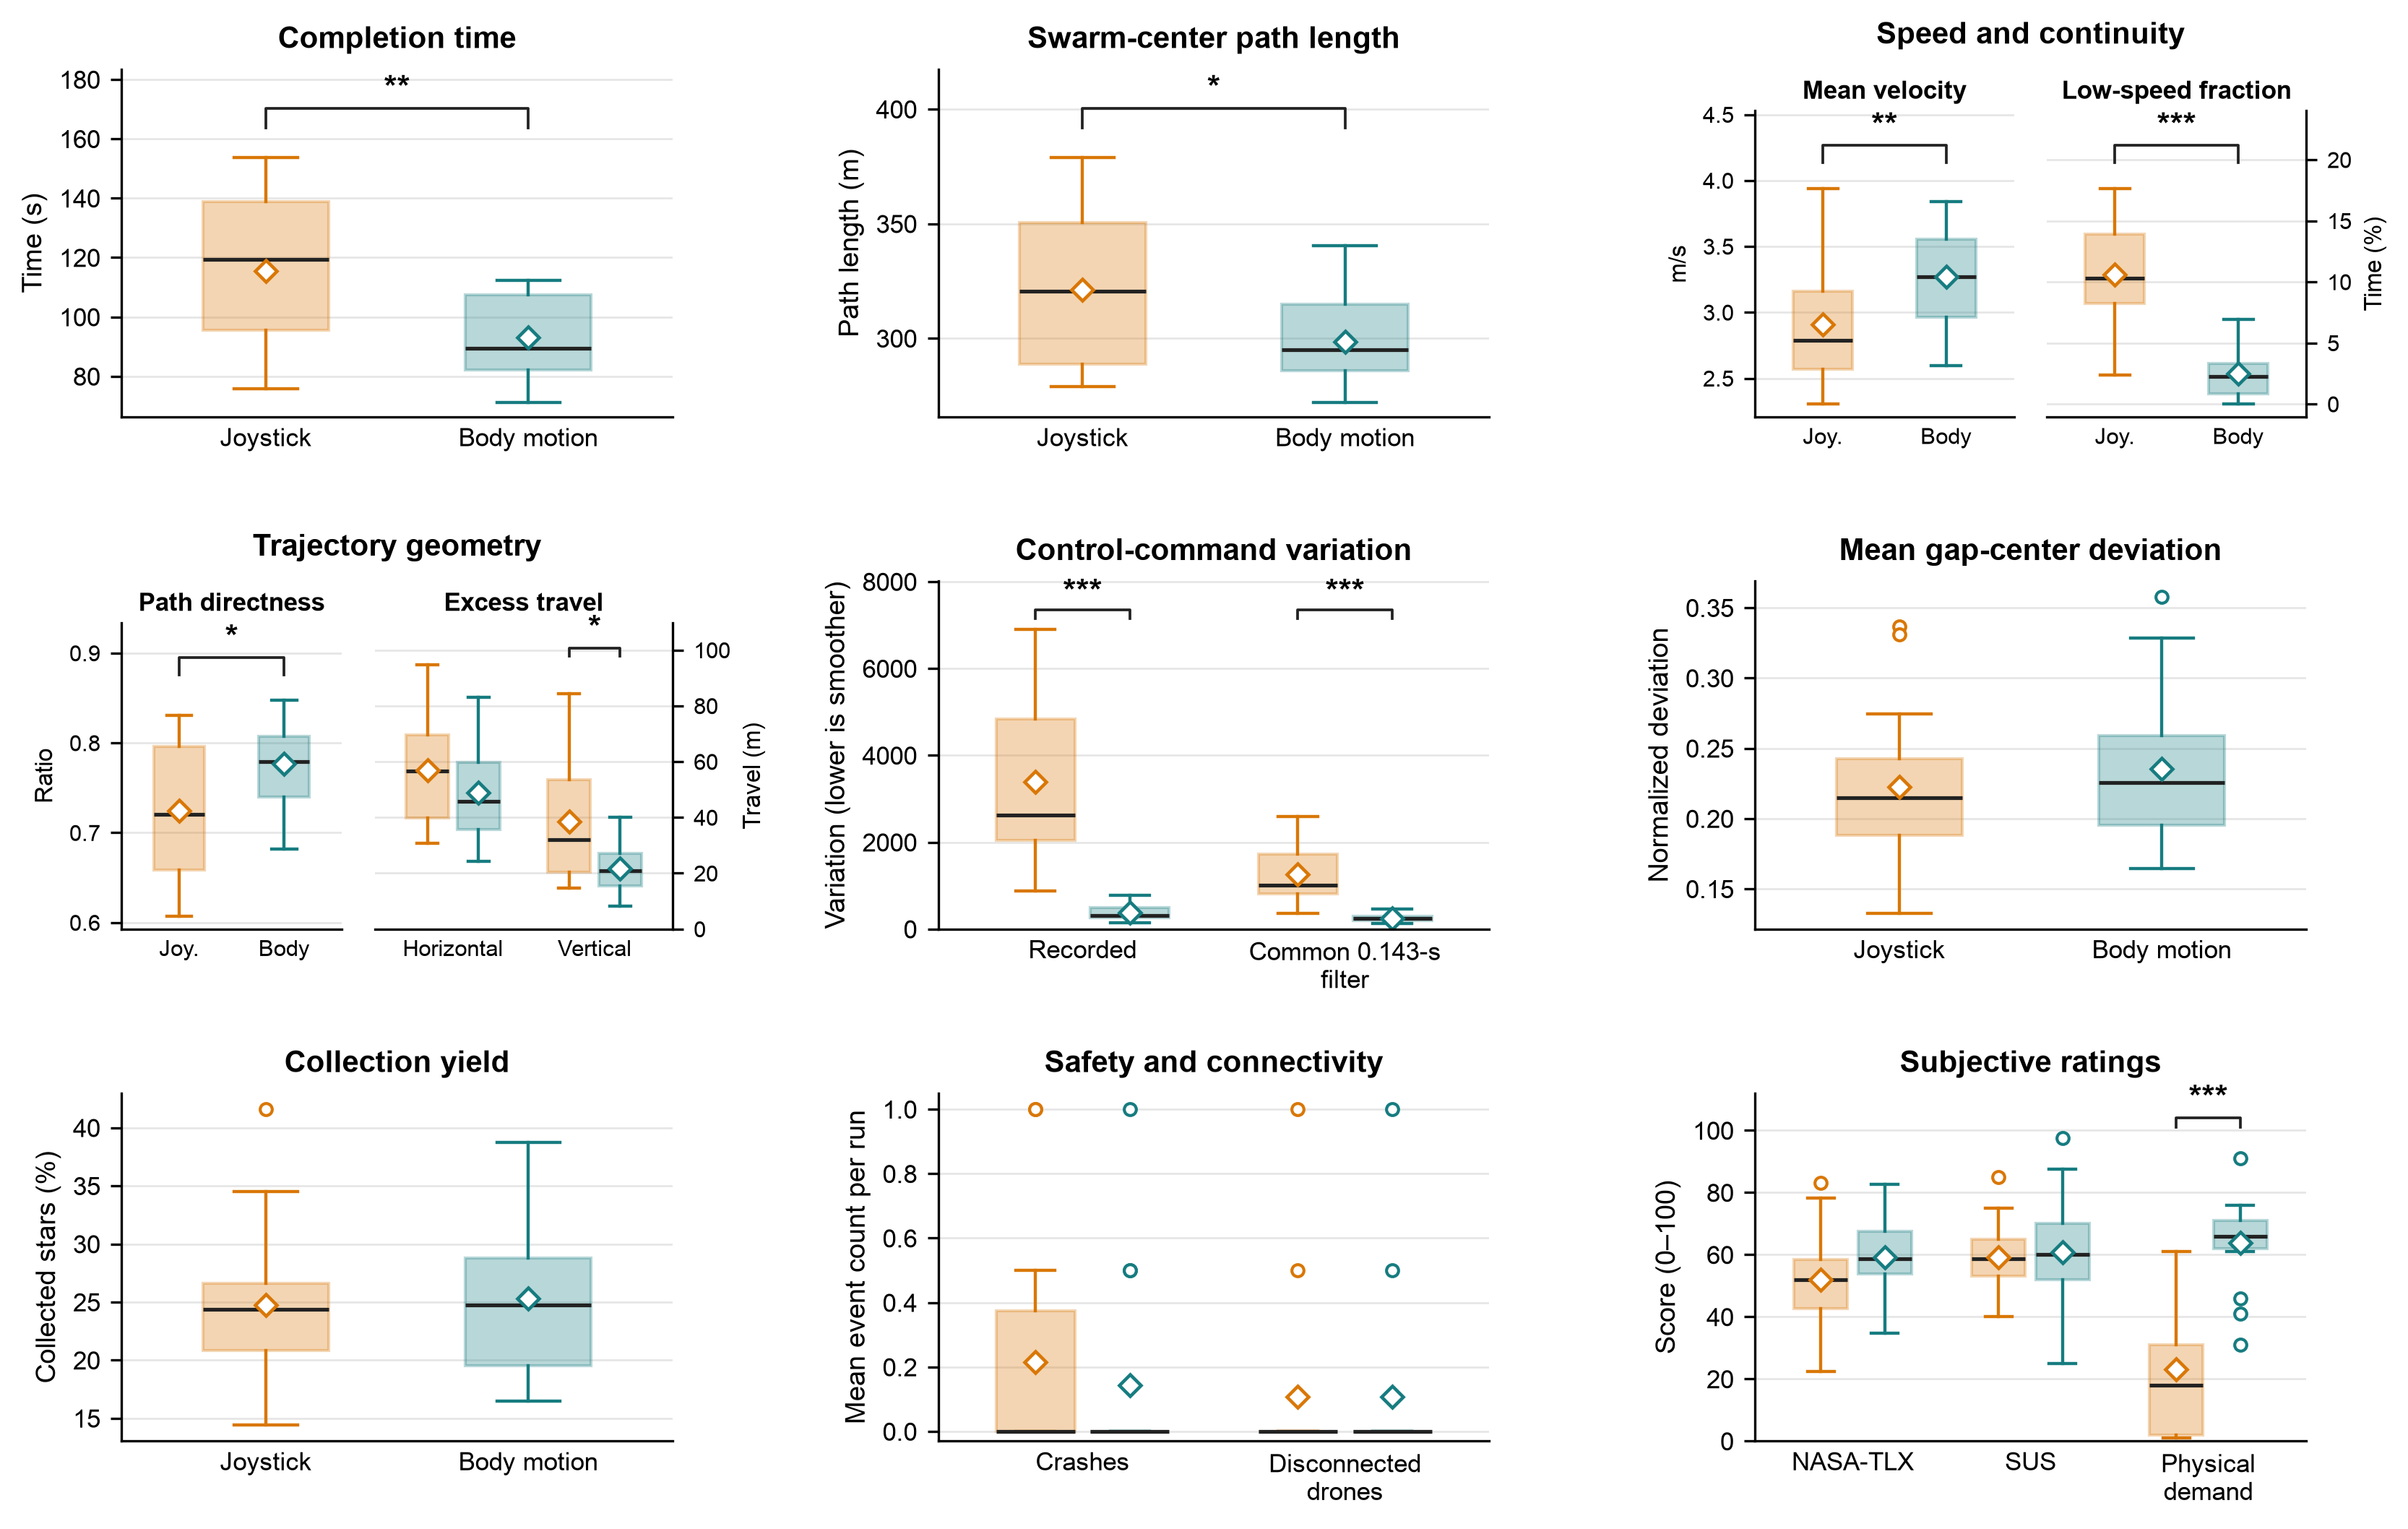
\includegraphics[width=\textwidth]{Figures/box.png}
\caption{\DIFaddFL{Participant-level outcomes for transmitter and body-motion control
($n=14$). 
%DIF >  Delivered-command variation and multi-DOF coordination are shown for the recorded pipelines.
Boxes show interquartile ranges with median lines; diamonds indicate means
and circles indicate outliers. Orange denotes transmitter and teal denotes body
motion. Stars mark Holm-adjusted paired comparisons
($*p<0.05$, $**p<0.01$, $***p<0.001$).}}
\label{fig:paired_results}
\end{figure*}

\DIFadd{For each segment, excess horizontal travel $H_{\mathrm{exc}}$ was the
horizontal path length in the $x$--$z$ plane minus the direct horizontal
displacement between its endpoints. Excess vertical travel
}\DIFaddend $V_{\mathrm{exc}}$ \DIFaddbegin \DIFadd{was the total absolute height change minus the direct
height change. Both measures were summed across the eight segments. Lower values indicate less excess motion}\DIFaddend .
\DIFdelbegin \DIFdel{Lower low-speed time, episode count, $C_{\perp}$, and
$V_{\mathrm{exc}}$, and higher straightness, indicated more continuous and
direct movement.
}\DIFdelend 

\DIFdelbegin \DIFdel{To characterize path directness, we performed a post-hoc gate-to-gate
decomposition. For each of the eight start--gate, gate--gate, and gate--finish
segments, $\hat{\mathbf{u}}_j$ denotes the unit vector along its endpoint chord. We
computed
}\begin{displaymath}
\DIFdel{\begin{aligned}
C_{\perp}
&=
\frac{
\sum_j\sum_k
\left\|
\Delta\mathbf{x}_{j,k}
-(\Delta\mathbf{x}_{j,k}^{\mathsf T}\hat{\mathbf{u}}_j)
 \hat{\mathbf{u}}_j
\right\|_2
}{
\sum_j\sum_k\lVert\Delta\mathbf{x}_{j,k}\rVert_2
},\\
V_{\mathrm{exc}}
&=
\sum_j
\left(
\sum_k |\Delta y_{j,k}|
-
|y_{j,K_j}-y_{j,1}|
\right).
\end{aligned}
\label{eq:trajectory_geometry}
}\end{displaymath}%DIFAUXCMD
\DIFdel{Lower $C_{\perp}$ indicates that a larger fraction of movement followed the direct three-dimensional segment directions.
Lower $V_{\mathrm{exc}}$
indicates less vertical reversal beyond the endpoint-to-endpoint height change.
We also examined the vertical component of gate-centering error separately}\DIFdelend \DIFaddbegin \emph{\DIFadd{Gate-centering error.}}
\DIFadd{For each gate, the swarm centroid was linearly interpolated at the gate-plane
crossing. Error was the in-plane distance $\sqrt{d_h^2+d_v^2}$ from the gate
center, where $d_h$ and $d_v$ are the horizontal and vertical offsets. We
averaged this distance across the seven gates.
}

\DIFadd{Collection yield was the fraction of the 316 available stars collected.
Crash count was the number of agents that crashed during a run.
Disconnection count was the number of agent-disconnection events recorded
during a run}\DIFaddend .

\emph{Delivered-command behavior.}
\DIFdelbegin \DIFdel{The five delivered commands---three translations, target spacing, and
view-yaw rate---were normalized by their implemented ranges to $\mathbf{q}_k\in[0,1]^5$. With }\DIFdelend \DIFaddbegin \DIFadd{Each command was normalized to $[0,1]$. Let $\mathbf{q}_k$ be the five-command
vector at sample $k$ and }\DIFaddend $\tau=t_M-t_1$ \DIFdelbegin \DIFdel{,
$\Delta\mathbf{q}_k=\mathbf{q}_{k+1}-\mathbf{q}_k$, and $\Delta t_k=t_{k+1}-t_k$, delivered-command variation was
}\DIFdelend \DIFaddbegin \DIFadd{the run duration. Delivered-command
variation was
}\DIFaddend \begin{equation}
E_{\mathrm{cmd}} = \frac{\tau}{5} \sum_{k=1}^{M-1} \DIFdelbegin \DIFdel{\frac{\lVert\Delta\mathbf{q}_k\rVert_2^2}{\Delta t_k}}\DIFdelend \DIFaddbegin \DIFadd{\frac{\lVert\mathbf{q}_{k+1}-\mathbf{q}_k\rVert_2^2}{t_{k+1}-t_k}}\DIFaddend .
\label{eq:command_metrics}
\end{equation}
Lower values indicate \DIFdelbegin \DIFdel{less variation in the commands supplied to
the swarm, not necessarily better performance}\DIFdelend \DIFaddbegin \DIFadd{smoother delivered commands.
}

\emph{\DIFadd{Multi-DOF coordination.}}
\DIFadd{Multi-DOF coordination was the percentage of active control time during which
at least two commands changed above $0.10~\mathrm{s^{-1}}$; active time required
at least one such command. Pairwise co-change applied the same definition to
each of the ten command pairs. Intervals with three or more changing commands
contributed to multiple pairs, so pairwise values were not additive}\DIFaddend . Because
the interfaces used different \DIFdelbegin \DIFdel{online filters, this metric characterizes }\DIFdelend \DIFaddbegin \DIFadd{temporal filtering, these measures describe }\DIFaddend the
complete delivered-command pipelines rather than intrinsic \DIFdelbegin \DIFdel{input smoothness }\DIFdelend \DIFaddbegin \DIFadd{smoothness or
intentional coordination}\DIFaddend .


\DIFdelbegin \emph{\DIFdel{Task accuracy and swarm integrity.}}
%DIFAUXCMD
\DIFdel{At the first ordered forward crossing of each gate, normalized gate-centering
error was
}\begin{displaymath}
\DIFdel{E_{\mathrm{gate}}=\frac{1}{7}\sum_{g=1}^{7}
\max\left(\frac{|h_g|}{W_g/2},\frac{|v_g|}{H_g/2}\right),
\label{eq:gate_error}
}\end{displaymath}%DIFAUXCMD
\DIFdel{where $h_g,v_g$ are offsets from the opening center and $W_g,H_g$ are its
dimensions.Values of zero and one indicate the opening center and edge,
respectively. We further measured unique-star collection yield, swarm survival
($1-N_{\mathrm{crash}}/15$), and the time-weighted fraction of surviving
agents in the largest connected component.
}\DIFdelend \DIFaddbegin \begin{figure}[!t]
\centering

\includegraphics[width=\columnwidth]
{\DIFaddFL{Figures/a.png}}
\caption{\DIFaddFL{Example Course 2 trajectories for one participant: (a) horizontal
paths and (b) gate-aligned heights under each interface. Thin lines show
non-focal agents, thick lines show the focal agent, and black markers show gate
locations and vertical openings.}}
\label{fig:trajectory_overlays}
\end{figure}
\DIFaddend 

\DIFdelbegin \emph{\DIFdel{Subjective measures.}}
%DIFAUXCMD
\DIFdel{NASA-TLX and SUS quantified workload and usability. Weighted TLX, its six
0--100 dimension ratings, and Raw TLX were analyzed. Interface preference and
relative motion sickness were summarized descriptively.
}%DIFDELCMD < 

%DIFDELCMD < %%%
\subsection{\DIFdel{Data Processing and Statistical Analysis}}
%DIFAUXCMD
\addtocounter{subsection}{-1}%DIFAUXCMD
%DIFDELCMD < \label{sec:statistical_analysis}
%DIFDELCMD < 

%DIFDELCMD < %%%
\DIFdelend %DIF >  =====================================================================
\DIFaddbegin \section{\DIFadd{Results}}
\DIFaddend All 56 runs were retained\DIFdelbegin \DIFdel{. Seven participants began with body motion and seven
with the transmitter. Metrics were computed from the native 15-Hz samples
without additional smoothing or resampling. The two courses were averaged within participantand interface}\DIFdelend \DIFaddbegin \DIFadd{; the two runs per interface were averaged for each
participant}\DIFaddend , yielding 14 paired observations. \DIFdelbegin %DIFDELCMD < 

%DIFDELCMD < %%%
\DIFdelend Interfaces were compared using exact two-sided Wilcoxon signed-rank tests (\DIFdelbegin \DIFdel{$\alpha=.05$). Holm correction was applied separately within the traversal,
task-outcome, primary-subjective, and TLX-dimension families. The post-hoc
trajectory family comprised $C_{\perp}$, $V_{\mathrm{exc}}$, and vertical
gate-centering error; the single delivered-command outcome required no
adjustment. Body-minus-transmitter mean differences are reported with
paired-bootstrap 95\% confidence intervals based on 20,000 resamples.
Sensitivity checks examined course, condition order, path sampling, common
additional filtering, and Raw TLX scoring.
}\DIFdelend \DIFaddbegin \DIFadd{$\alpha=0.05$)~\mbox{%DIFAUXCMD
\cite{wilcoxon1945ranking}}\hskip0pt%DIFAUXCMD
, with Holm adjustment within outcome families~\mbox{%DIFAUXCMD
\cite{holm1979procedure}}\hskip0pt%DIFAUXCMD
.
}\DIFaddend 

%DIF <  =====================================================================
\DIFdelbegin \section{\DIFdel{Results}}
%DIFAUXCMD
\addtocounter{section}{-1}%DIFAUXCMD
%DIFDELCMD < 

%DIFDELCMD < %%%
\DIFdel{Paired analyses included all 14 participants and are presented below.
}%DIFDELCMD < 

%DIFDELCMD < \begin{figure}[!tb]
%DIFDELCMD < \centering
%DIFDELCMD < 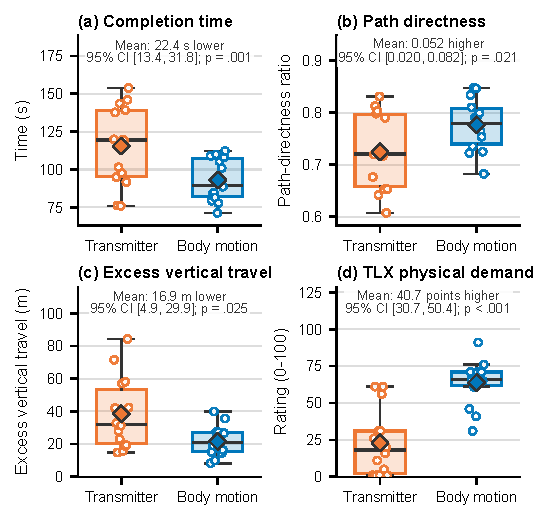
\includegraphics[width=\columnwidth]{Figures/fig_paired_results_2x2.pdf}
%DIFDELCMD < %%%
%DIFDELCMD < \caption{%
{%DIFAUXCMD
\DIFdelFL{Paired outcomes: (a) completion time, (b) 3-D cross-track
fraction, (c) excess vertical travel, and (d) TLX physical demand. Lines
connect interfaces, open symbols denote participants, and diamonds denote
means. Annotations report body-minus-transmitter differences, bootstrap 95\%
CIs, and Holm-adjusted $p_{\mathrm H}$ values. Panels (b,c) are post hoc.}}
%DIFAUXCMD
%DIFDELCMD < \label{fig:paired_results}
%DIFDELCMD < \end{figure}
%DIFDELCMD < 

%DIFDELCMD < %%%
\DIFdelend \emph{Traversal efficiency.}
\DIFdelbegin \DIFdel{Body motion reduced completion time from 115.4 to 93.0~s, a }\DIFdelend \DIFaddbegin \DIFadd{Completion time was }\DIFaddend 19.4\% \DIFdelbegin \DIFdel{reduction
}\DIFdelend \DIFaddbegin \DIFadd{lower with body motion, a mean reduction of
22.4~s }\DIFaddend (\DIFdelbegin \DIFdel{$\Delta=-22.4$~s ; 95\% CI $[-31.8,-13.4]$;
$p_{\mathrm H}=.001$}\DIFdelend \DIFaddbegin \DIFadd{Holm-adjusted $p=0.001$}\DIFaddend ); 13 of 14 participants were faster\DIFdelbegin \DIFdel{(Fig. ~\ref{fig:paired_results}(a)). Paths were }\DIFdelend \DIFaddbegin \DIFadd{. Centroid
path length was }\DIFaddend 7.0\% shorter (\DIFdelbegin \DIFdel{298.6 versus 321.1~m; $p_{\mathrm H}=.011$}\DIFdelend \DIFaddbegin \DIFadd{$p=0.011$}\DIFaddend ), and mean speed was 12.5\% higher
(\DIFdelbegin \DIFdel{3.27 versus 2.91~m/s; $p_{\mathrm H}=.001$}\DIFdelend \DIFaddbegin \DIFadd{$p=0.001$}\DIFaddend ).

\DIFdelbegin \DIFdel{Post hoc decomposition indicated more continuous and direct motion. Time below
0.5~m/s decreased from 13.23 to 2.45~s ($\Delta=-10.78$~s; 95\% CI
$[-14.30,-7.42]$; $p_{\mathrm H}<.001$), and sustained low-speed episodes
decreased from 6.68 to 1.39 per trial ($p_{\mathrm H}<.001$).
Gate-to-gate straightness increased from 0.725 to 0.776
($\Delta=0.052$; 95\% CI $[0.021,0.082]$;
$p_{\mathrm H}=.011$). }%DIFDELCMD < 

%DIFDELCMD < %%%
\emph{\DIFdel{Trajectory geometry.}}
%DIFAUXCMD
\DIFdel{The 3-D cross-track fraction decreased by 8.6\%, from 0.552 to 0.505
($\Delta=-0.047$; 95\% CI $[-0.070,-0.023]$;
$p_{\mathrm H}=.007$), with lower values for 12 of 14 participants
(Fig.~\ref{fig:paired_results}(b)).
Excess vertical travel decreased by
44.0\% , from 38.5 to 21.6~m($\Delta=-16.9$~m; 95\% CI
$[-30.1,-4.9]$; $p_{\mathrm H}=.049$;
Fig.~\ref{fig:paired_results}(c))}\DIFdelend \DIFaddbegin \emph{\DIFadd{Trajectory characteristics.}}
\DIFadd{Path directness increased by 0.052 (Holm-adjusted $p=0.032$). Excess vertical
travel decreased by 44.0\%, corresponding to 16.9~m (Holm-adjusted $p=0.049$)}\DIFaddend .
\DIFaddbegin \DIFadd{Excess horizontal travel was 14.2\% lower with body motion (48.8 versus
56.8~m), but no clear difference was detected (mean difference $-8.0$~m,
$p=0.153$). }\DIFaddend Figure~\ref{fig:trajectory_overlays} \DIFdelbegin \DIFdel{shows the corresponding horizontal paths and height profiles}\DIFdelend \DIFaddbegin \DIFadd{illustrates these patterns}\DIFaddend .

\DIFdelbegin %DIFDELCMD < \begin{figure*}[!t]
%DIFDELCMD < \vspace{-2mm}
%DIFDELCMD < %%%
\DIFdelendFL \DIFaddbeginFL \begin{figure}[!t]
\DIFaddendFL \centering
\DIFdelbeginFL %DIFDELCMD < \includegraphics[width=\linewidth]
%DIFDELCMD < %%%
\DIFdelendFL \DIFaddbeginFL \includegraphics[width=\columnwidth]
\DIFaddendFL {Figures/fig\DIFdelbeginFL \DIFdelFL{_trajectory_overlays_height_mean_max.pdf}\DIFdelendFL \DIFaddbeginFL \DIFaddFL{_pairwise_dof_cochange.png}\DIFaddendFL }
\DIFdelbeginFL %DIFDELCMD < \vspace{-1mm}
%DIFDELCMD < %%%
\DIFdelendFL \caption{\DIFdelbeginFL \DIFdelFL{Centroid trajectories }\DIFdelendFL \DIFaddbeginFL \DIFaddFL{Exploratory pairwise command co-change }\DIFaddendFL for \DIFdelbeginFL \DIFdelFL{both courses. Panels }\DIFdelendFL (a\DIFdelbeginFL \DIFdelFL{,b}\DIFdelendFL ) \DIFdelbeginFL \DIFdelFL{show top views,
}\DIFdelendFL \DIFaddbeginFL \DIFaddFL{body-motion }\DIFaddendFL and
\DIFdelbeginFL \DIFdelFL{panels }\DIFdelendFL (\DIFdelbeginFL \DIFdelFL{c,d}\DIFdelendFL \DIFaddbeginFL \DIFaddFL{b}\DIFaddendFL ) \DIFdelbeginFL \DIFdelFL{show gate-aligned height profiles}\DIFdelendFL \DIFaddbeginFL \DIFaddFL{transmitter control}\DIFaddendFL . \DIFdelbeginFL \DIFdelFL{Thin curves are individual
runs, thick curves are interface medians, and dashed lines indicate }\DIFdelendFL \DIFaddbeginFL \DIFaddFL{Off-diagonal cells show }\DIFaddendFL the \DIFdelbeginFL \DIFdelFL{mean
run-wise maximum height}\DIFdelendFL \DIFaddbeginFL \DIFaddFL{percentage of active
control time during which both commands were active; diagonal cells show
single-command activity}\DIFaddendFL . \DIFaddbeginFL \DIFaddFL{Values were averaged across participants ($n=14$)
using a shared color scale.}\DIFaddendFL }
\DIFdelbeginFL %DIFDELCMD < \label{fig:trajectory_overlays}
%DIFDELCMD < \vspace{-2mm}
%DIFDELCMD < \end{figure*}
%DIFDELCMD < %%%
\DIFdelend \DIFaddbegin \label{fig:dof_pairwise}
\end{figure}
\DIFaddend 

\emph{Delivered-command behavior.}
\DIFdelbegin \DIFdel{Delivered-command }\DIFdelend \DIFaddbegin \DIFadd{Command }\DIFaddend variation was 88.8\% lower \DIFdelbegin \DIFdel{in the implemented body-motion
pipeline ($p_{\mathrm H}<.001$).
Applying the
same additional 0.143-s
low-pass filter to both delivered streams preserved an approximately 80.0\%
reduction. Because pre-filter body commands were
not logged, this comparison
characterizes the complete pipelines rather than input modality alone}\DIFdelend \DIFaddbegin \DIFadd{with body motion (Holm-adjusted $p<0.001$).
Multi-DOF coordination was 22.5 percentage points higher ($p<0.001$), with the
same direction for all participants. Pairwise co-change was higher for seven of
ten command pairs (Fig.~\ref{fig:dof_pairwise}). The largest differences were
vertical--forward (19.3\% versus 5.5\%), forward--spacing (10.5\% versus 0.3\%),
and vertical--spacing (10.0\% versus 0.1\%; $p=0.001$ each).
Lateral--spacing was also higher (8.1\% versus 0.5\%), whereas the three
translation--yaw pairs did not differ after Holm correction}\DIFaddend .

\emph{Task \DIFdelbegin \DIFdel{outcomes}\DIFdelend \DIFaddbegin \DIFadd{performance and swarm integrity}\DIFaddend .} 
No \DIFdelbegin \DIFdel{clear interface difference was detected in gate centering, collection ,
survival, or largest-component retention. 
Survival and connectivity remained
near ceiling with both interfaces; these results do not establish equivalent
task performance or safety.
}\DIFdelend \DIFaddbegin \DIFadd{differences were detected in gate-centering error, collection yield, crash count, or disconnection-event count (Holm-adjusted \(p=1.000\) for all four outcomes). 
}\DIFaddend 

\DIFdelbegin \emph{\DIFdel{Subjective outcomes.}}
%DIFAUXCMD
\DIFdel{Weighted TLX showed no clear interface difference ($\Delta=7.2$; 95\% CI
$[-5.5,20.2]$),
nor did SUS. Physical demand, however, increased from 23.0
to 63.7 and was higher }\DIFdelend \DIFaddbegin \emph{\DIFadd{Subjective experience.}} 
\DIFadd{Overall weighted NASA-TLX and SUS scores did not differ between conditions
(mean differences 7.2 and 1.6; Holm-adjusted $p=0.482$ and $p=0.491$,
respectively). However, all 14 participants reported higher physical demand
}\DIFaddend with body motion \DIFdelbegin \DIFdel{for all participants
($\Delta=40.7$; 95\% CI $[30.7,50.4]$;
$p_{\mathrm H}<.001$; Fig.~\ref{fig:paired_results}(d)).
Eight participants
preferred body motion, five preferred the transmitter, and one reported no
preference. Motion-sickness reports were
mixed }\DIFdelend \DIFaddbegin \DIFadd{(mean increase 40.7 points; Holm-adjusted $p<0.001$)}\DIFaddend .
\DIFaddbegin \DIFadd{Interface preference was divided, and relative motion-sickness responses were
mixed (Fig.~\ref{fig:subjective_responses}).
}\DIFaddend 

\DIFdelbegin %DIFDELCMD < \FloatBarrier
%DIFDELCMD < %%%
\DIFdelend \DIFaddbegin \begin{figure}[!b]
\centering

\includegraphics[width=\columnwidth]
{\DIFaddFL{Figures/fig_subjective_responses.png}}
\caption{\DIFaddFL{Comparative responses after both interface blocks (n = 14). The
upper bar shows interface preference, and the lower bar shows the interface
associated with greater motion sickness. Neutral denotes no preference in
the upper bar and no difference in motion sickness in the lower bar. Counts
are descriptive; no inferential comparison was performed.}}
\label{fig:subjective_responses}
\end{figure}
\DIFaddend 

%DIF <  =====================================================================
%DIF >  ====================================================================
\DIFaddbegin 

\DIFaddend \section{Discussion}
\DIFaddbegin \DIFadd{The implemented body-motion interface improved traversal efficiency and path directness in the tested FPV swarm-navigation task, with the trajectory
improvement concentrated in the vertical rather than the horizontal dimension. Two observations may help explain this pattern. First, multi-DOF coordination was higher with body motion than with the transmitter, consistent with participants' reports that they could adjust several commands simultaneously rather than moving between transmitter controls. This aligns with the distinction between integral and separable input
\mbox{%DIFAUXCMD
\cite{jacob1994integrality,zhai1998quantifying}}\hskip0pt%DIFAUXCMD
. Second, body motion reduced delivered-command variation, which may have supported more continuous forward motion and fewer corrections. These associations are consistent with the measured efficiency gains but do not establish causation.
}\DIFaddend 

\DIFdelbegin \DIFdel{Body motion enabled faster and more direct traversal : participants completed
the courses 19.4\% faster, followed shorter paths, spent less time moving
slowly, and showed lower cross-track motion. Excess vertical travel was also
lower, although this post hoc effect was close to the significance threshold.
These related measures indicate that the advantage arose through more continuous }\DIFdelend \DIFaddbegin \DIFadd{Several participants reported that leaning forward involuntarily lowered their
hands, changed the altitude command, }\DIFaddend and \DIFdelbegin \DIFdel{direct movement, but they are not independent confirmations of
the completion-time result}\DIFdelend \DIFaddbegin \DIFadd{required a correction, although they adapted to this coupling quickly. This mechanical coupling could increase the measured coordination index without reflecting intentional concurrent control. The pairwise results are consistent with this concern: the differences covered several command pairs and were largest for vertical and forward control, rather than being confined to lateral motion and spacing. However, task demands and interface-specific filtering could also produce co-change, so the matrix does not identify its cause. Physical arm support
\mbox{%DIFAUXCMD
\cite{rognon2018flyjacket} }\hskip0pt%DIFAUXCMD
or measuring hand height relative to the torso could help decouple these commands}\DIFaddend .

\DIFdelbegin \DIFdel{Both interfaces exposed the same five continuous DOF; body motion changed
their
physical allocation rather than their number. Delivered commands were less variable with body motion. However, the interfaces
differed in hardware, calibration, mapping, and filtering. }\DIFdelend The \DIFdelbegin \DIFdel{results therefore compare
the implemented end-to-end systems and do not isolate the effects of body input, DOF allocation, or signal processing.
}%DIFDELCMD < 

%DIFDELCMD < %%%
\DIFdel{The }\DIFdelend efficiency advantage was not accompanied by a detected \DIFdelbegin \DIFdel{difference in gate
centering, collection , survival, or connectivity. This provides no evidence of a measured task-performance trade-off, but ceiling effects and the small sample
prevent claims of equivalence or comparable safety. Body motion also imposed a
clear physical cost,
despite no detected difference in total TLX or SUS. Arm support or smaller-excursion gains may reduce effort
\mbox{%DIFAUXCMD
\cite{rognon2018flyjacket}}\hskip0pt%DIFAUXCMD
, while formation-clearance feedback could
improve
spatial awareness \mbox{%DIFAUXCMD
\cite{tsykunov2019swarmtouch}}\hskip0pt%DIFAUXCMD
}\DIFdelend \DIFaddbegin \DIFadd{loss of task
accuracy or swarm integrity: gate-centering error, collection yield, crash
count, and disconnection events did not differ between interfaces. However,
the absence of a detected difference does not establish equivalence.
}

\DIFadd{The larger vertical reversals illustrated in Fig.~\ref{fig:trajectory_overlays}(b) are consistent with repeated altitude corrections under transmitter control, although the figure alone does not establish their cause. The fixed throttle gain may have been too sensitive for some participants. In addition, the body-motion altitude command was
individually calibrated and smoothed, whereas the transmitter command was
neither personalized nor additionally filtered. The results therefore compare
the complete implemented interfaces and cannot be attributed solely to input
modality. Future comparisons should match temporal filtering and evaluate
participant-specific transmitter gains and alternative command mappings.
Because we tested one body-motion mapping and one transmitter configuration,
the findings characterize these implementations rather than body-motion
control in general.
}

\DIFadd{The body-motion interface required more physical demand, although overall
workload was unchanged. All 14 participants rated it as more physically
demanding, while lower ratings on the remaining TLX dimensions offset this
strain. Preference remained split, suggesting that the added physical demand
reduced the appeal of the efficiency gain for some operators. Beyond
decoupling torso and arm commands, increasing the shoulder-motion gains could
reduce the required movement range at the cost of fine control accuracy.
}

\DIFadd{Because both conditions used only a rear-focal FPV, the observed differences
may not generalize to front-focal or simultaneous multi-view configurations.
Viewpoint and input mapping may interact and should be examined in a factorial
study.
}

\DIFadd{Concurrent control of several commands may allow a single operator to navigate
more complex environments. By translating the swarm, changing its altitude and
spacing, and redirecting the viewpoint simultaneously, the interface could
support tighter, more irregular, or dynamically changing three-dimensional
spaces}\DIFaddend .

These findings extend upper-body control from individual aerial robots
\DIFaddbegin \DIFadd{\mbox{%DIFAUXCMD
\cite{rognon2018flyjacket,miehlbradt2018datadriven,macchini2024datadriven}
}\hskip0pt%DIFAUXCMD
}\DIFaddend and externally viewed formations
\DIFdelbegin \DIFdel{\mbox{%DIFAUXCMD
\cite{rognon2018flyjacket,miehlbradt2018datadriven,
macchini2024datadriven,macchini2021personalized}
}\hskip0pt%DIFAUXCMD
to }\DIFdelend \DIFaddbegin \DIFadd{\mbox{%DIFAUXCMD
\cite{macchini2021personalized,tsykunov2019swarmtouch,kratky2025gesture}
}\hskip0pt%DIFAUXCMD
to continuous five-DOF swarm control from a }\DIFaddend rear-focal FPV\DIFdelbegin \DIFdel{swarm teleoperation.
}%DIFDELCMD < 

%DIFDELCMD < %%%
\DIFdel{Future work should use larger samples, counterbalanced courses,
longer exposure, and harder tasks; record commands before and after processing;
and match or ablate interface mappings and filtering. Physical-swarm studies
are needed to test whether the efficiency advantage persists under
communication }\DIFdelend , \DIFdelbegin \DIFdel{aerodynamic, }\DIFdelend and \DIFdelbegin \DIFdel{safety constraints}\DIFdelend \DIFaddbegin \DIFadd{complement
transmitter-based FPV swarm control~\mbox{%DIFAUXCMD
\cite{ben_focaldrone}}\hskip0pt%DIFAUXCMD
. The swarm was
simulated, so communication latency, aerodynamic disturbances, and real-world
safety limits were absent; validation with physical swarms is therefore
necessary}\DIFaddend .

%DIF <  \begin{figure}[t]
%DIF <  \centering
%DIF <  \includegraphics[width=\columnwidth]{Figures/fig_traj_comparison.png}
%DIF <  \caption{LOL TRAJ LOL}
%DIF <  \label{fig:paired_results}
%DIF <  \end{figure}
% =====================================================================
\DIFdelbegin \section{\DIFdel{Conclusion}}
%DIFAUXCMD
\addtocounter{section}{-1}%DIFAUXCMD
\DIFdelend 

\DIFaddbegin \section{\DIFadd{Conclusion}}
\DIFaddend We presented a participant-calibrated upper-body interface for continuous
five-DOF FPV swarm teleoperation. In a 14-participant within-subject study,
the \DIFdelbegin \DIFdel{complete }\DIFdelend \DIFaddbegin \DIFadd{implemented }\DIFaddend body-motion \DIFdelbegin \DIFdel{system }\DIFdelend \DIFaddbegin \DIFadd{interface }\DIFaddend reduced completion time by 19.4\% relative to a transmitter \DIFdelbegin \DIFdel{, with 7.0\% shorter paths, higher mean speed, and }\DIFdelend \DIFaddbegin \DIFadd{and produced more direct trajectories with }\DIFaddend lower delivered-command variation\DIFdelbegin \DIFdel{. However, physical demand increased, while no differences were detected }\DIFdelend \DIFaddbegin \DIFadd{, at the
cost of higher physical demand and with no detected differences }\DIFaddend in task
accuracy, swarm integrity, total workload, or usability\DIFdelbegin \DIFdel{; these
null results do not establish equivalence. Matched-processing and physical-swarm studies are needed to isolate modality effects and determine whether the efficiency advantage generalizes beyond the
tested simulated 15-agent rear-FPV task}\DIFdelend \DIFaddbegin \DIFadd{. Validation on physical
swarms remains necessary. For first-person-view swarm teleoperation, these
results support distributing the command dimensions that vary together across
separate body segments rather than across controls on a single handheld device. They also suggest that referencing hand height to the torso rather than to the
world would reduce the postural coupling that participants reported}\DIFaddend .

% =====================================================================
\DIFaddbegin 

\section*{\DIFadd{Acknowledgment}}
\DIFadd{The authors thank Benjamin Jarvis for constructive feedback on the manuscript, Pablo Palle for contributions to the simulation framework, and Gabriel Taieb for helping test the experimental protocol.
}

\DIFaddend \bibliographystyle{IEEEtran}
\bibliography{references}

\end{document}
